\documentclass{beamer}

%\includeonlyframes{current}

\usepackage[T1]{fontenc}
\usepackage[utf8]{inputenc}
\usepackage[american]{babel}
\usepackage{amsmath,amssymb,amsthm}
\usepackage{tikz}
\usepackage[backend=biber,citestyle=authoryear-comp,bibstyle=beamer,doi=false,isbn=false,url=false,maxnames=10]{biblatex}
\bibliography{defeo}

\mode<presentation>{%
  \usetheme{Boadilla}
}
\beamertemplatenavigationsymbolsempty

\usepackage{sourcesanspro}
\usepackage[amssymb,amsfonts]{concmath}
\usefonttheme[onlymath]{serif}

\renewcommand{\emph}[1]{{\usebeamercolor[fg]{structure}#1}}

%\let\footcite\footnote

\newcommand{\C}{\mathbb{C}}
\newcommand{\R}{\mathbb{R}}
\newcommand{\Z}{\mathbb{Z}}
\newcommand{\N}{\mathbb{N}}
\newcommand{\Q}{\mathbb{Q}}
\newcommand{\F}{\mathbb{F}}
\renewcommand{\P}{\mathbb{P}}
\renewcommand{\O}{\mathcal{O}}
\newcommand{\tildO}{\mathcal{\tilde{O}}}
\newcommand{\End}{\operatorname{End}}
\newcommand{\chr}{\operatorname{char}}
\newcommand{\Cl}{\operatorname{Cl}}
\renewcommand{\a}{{\mathfrak{a}}}
\renewcommand{\b}{{\mathfrak{b}}}
\newcommand{\cyc}[1]{{\langle #1 \rangle}}
\newcommand{\ord}{\operatorname{ord}}

\usetikzlibrary{arrows,matrix,decorations,decorations.text,decorations.pathmorphing,calc}

\pgfkeys{/triangle/.code=\tikzset{x={(-0.5cm,-0.866cm)},y={(1cm,0cm)}}}
\pgfkeys{/lattice/.code n args={4}{\tikzset{cm={#1,#2,#3,#4,(0,0)}}}}

\newcommand{\axes}[4]{
  \clip (#1,#3) rectangle (#2,#4);
  \draw [thin, gray, -latex] (#1,0) -- (#2,0);% Draw x axis
  \draw [thin, gray, -latex] (0,#3) -- (0,#4);% Draw y axis
}

\newcommand{\lattice}[2]{
  \draw[style=help lines,dashed] (#1-1,#1-1) grid[step=1] (#2+1,#2+1);
  \foreach \x in {#1,...,#2}{
    \foreach \y in {#1,...,#2}{
      \node[draw,circle,inner sep=2pt,fill] at (\x,\y) {};
      % Places a dot at those points
    }
  }
}

\newcommand{\bl}[1]{\textcolor{blue}{#1}}
\newcommand{\rd}[1]{\textcolor{red}{#1}}
\newcommand{\gr}[1]{\textcolor{green}{#1}}

% This command defines a triangle of dots of given height
\newcommand{\dottriangle}[2][\i-\j]{%
  \foreach \i in {0,...,#2} {%
    \foreach \j in {0,...,\i} {%
      \draw(\i,\j) node{#1};%
    }%
  }}


\title{Isogeny graphs in cryptography}
\author[Luca De Feo]{Luca De Feo}
\date[Mar 19--23, 2018 --- Post-Scryptum]{March 19--23, 2018, Post-Scryptum Spring School,
  Les 7 Laux
}
\institute[U Paris Saclay]{Université Paris Saclay, UVSQ \& Inria}

\begin{document}

\frame[plain]{
  \begin{tikzpicture}[remember picture,overlay]
    \node[at=(current page.center), opacity=0.7] {
      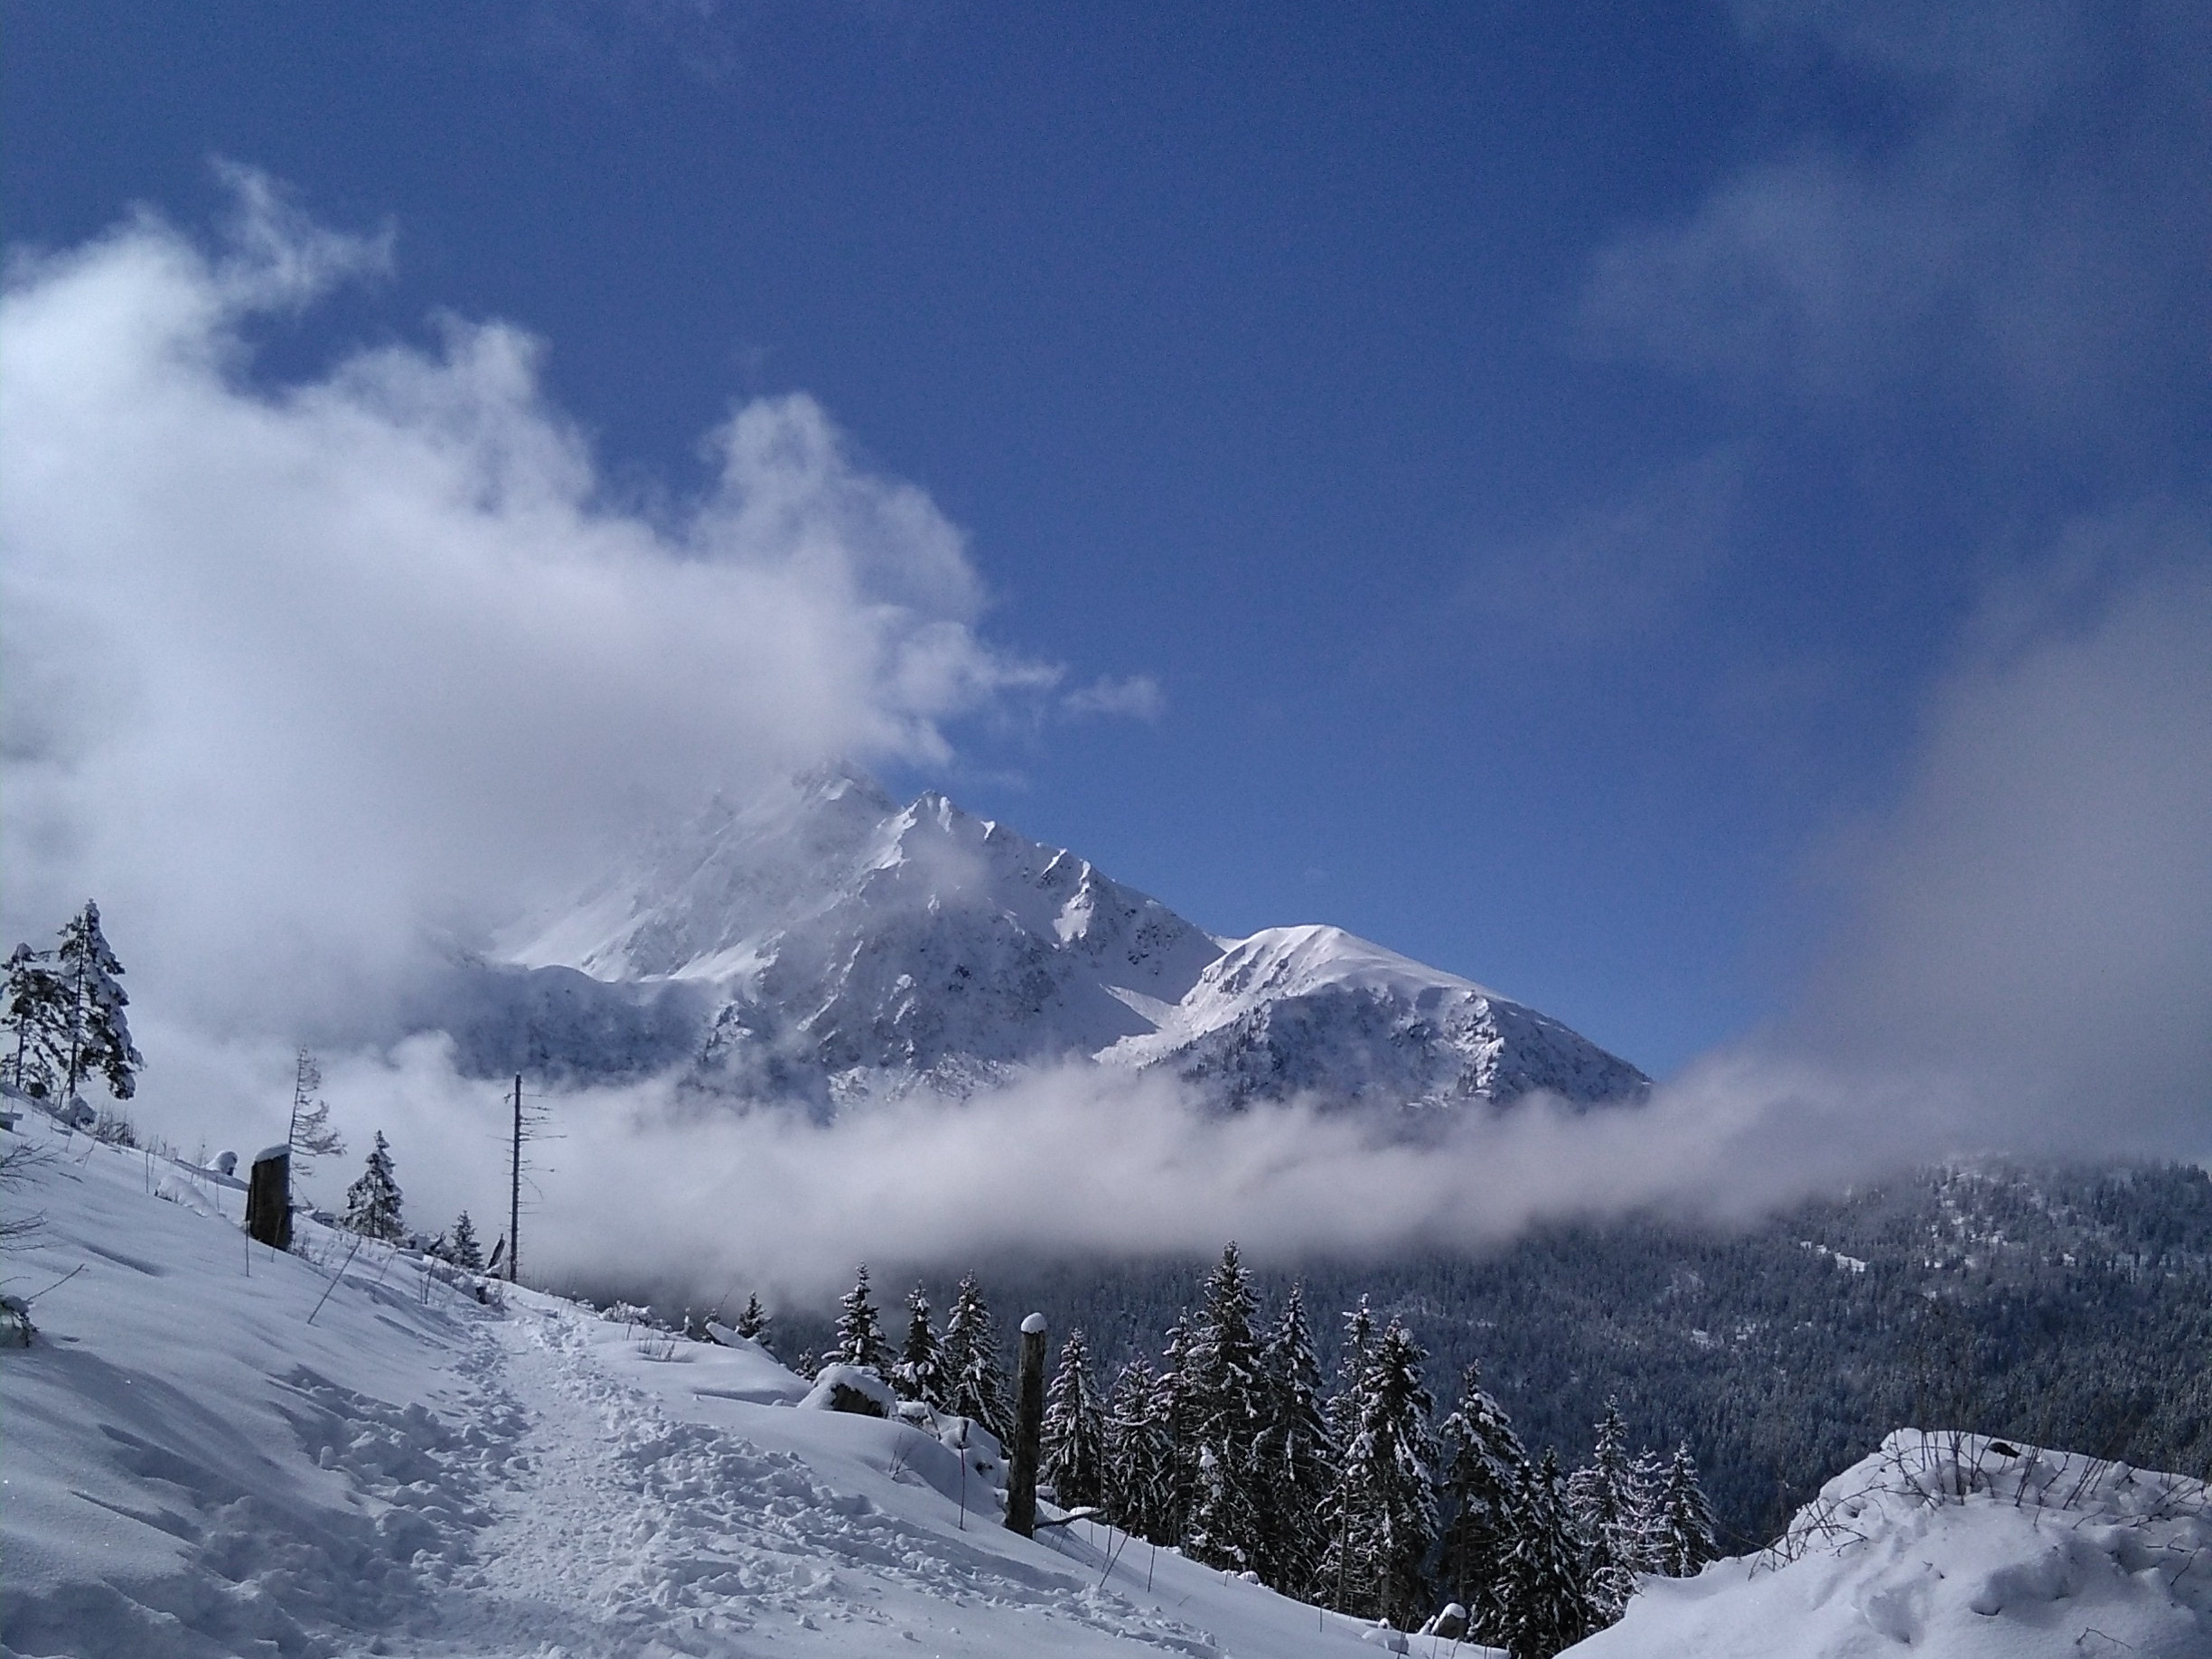
\includegraphics[width=1.2\paperwidth]{7laux.jpg}
    };
    \node[yshift=1em,xshift=5em,at=(current page.south west)]{\tiny Photo courtesy of Elisa Lorenzo-García};
  \end{tikzpicture}
  \vspace{-1.1cm}
  {\bf \titlepage}
  \vspace{0.5cm}
  \begin{center}
    Slides online at~~~\emph{\url{http://defeo.lu/docet/}}
  \end{center}
}

%% 

\begin{frame}
  \frametitle{Overview}
  \tableofcontents  
\end{frame}

%%
%% 

\section{Foundations}

\subsection{Elliptic curves}

\begin{frame}{Projective space}
  \begin{definition}[Projective space]
    Let $\bar{k}$ an algebraically closed field, the \emph{projective
      space} $\P^n(\bar{k})$ is the set of non-null $(n+1)$-tuples
    $(x_0,\dots,x_n)\in \bar{k}^n$ modulo the equivalence relation
    \[(x_0,\dots,x_n) \sim (\lambda x_0, \dots, \lambda x_n) \qquad
      \text{with $\lambda\in \bar{k}\setminus\{0\}$}.\]
    A class is denoted by $(x_0:\cdots:x_n)$.
  \end{definition}

  \centering
  \includegraphics[height=0.5\textheight]{camera-obscura.jpg}
\end{frame}

%%

\begin{frame}{Weierstrass equations}
  \begin{columns}
    \begin{column}{0.4\textwidth}
      Let $k$ be a field of characteristic $\ne 2,3$.

      An \emph{elliptic curve \textit{defined over $k$}} is the locus
      in $\P^2(\bar{k})$ of an equation
      \[\emph{Y^2Z = X^3 + aXZ^2 + bZ^3},\]
      where $a,b\in k$ and $4a^3+27b^2\ne 0$.

      \begin{itemize}
      \item<2-> $\O=(0:1:0)$ is the \emph{point at infinity};
      \item<3-> $y^2 = x^3 + ax + b$ is the \emph{affine equation}.
      \end{itemize}
    \end{column}
    \begin{column}{0.6\textwidth}
      \begin{center}
        \begin{tikzpicture}[domain=-2.4566:4,samples=100,yscale=1/2]
          \draw plot (\x,{sqrt(\x*\x*\x-4*\x+5)});
          \draw plot (\x,{-sqrt(\x*\x*\x-4*\x+5)});

          \draw[thin,gray,-latex] (0,-7) -- (0,7);
          \draw[thin,gray,-latex] (-3,0) -- (4,0);
        \end{tikzpicture}
      \end{center}
    \end{column}
  \end{columns}
\end{frame}

%%

\begin{frame}{The group law}
  \begin{columns}
    \begin{column}{0.4\textwidth}
      \begin{block}{Bezout's theorem}
        Every line cuts $E$ in exactly three points (counted with
        multiplicity).
      \end{block}

      Define a \emph{group law} such that any three colinear points
      add up to zero.

      \begin{itemize}
      \item<2-> The law is \emph{algebraic}\\ (it has \textit{formulas});
      \item<3-> The law is \emph{commutative};
      \item<3-> $\O$ is the \emph{group identity};
      \item<3-> \emph{Opposite points} have the same $x$-value.
      \end{itemize}
    \end{column}
    \begin{column}{0.6\textwidth}
      \begin{center}
        \begin{tikzpicture}[domain=-2.4566:4,samples=100,yscale=1/2]
          \draw plot (\x,{sqrt(\x*\x*\x-4*\x+5)});
          \draw plot (\x,{-sqrt(\x*\x*\x-4*\x+5)});

          \draw[thin,gray,-latex] (0,-7) -- (0,7);
          \draw[thin,gray,-latex] (-3,0) -- (4,0);
          \draw (-3,1) -- (4,8/3+3);
          \begin{scope}[every node/.style={draw,circle,inner sep=1pt,fill},cm={1,2/3,0,0,(0,3)}]
            \node at (-2.287980,0) {};
            \node at (-0.535051,0) {};
            \node at (3.267475,0) {};
          \end{scope}
          \begin{scope}[every node/.style={yshift=0.3cm},cm={1,2/3,0,0,(0,3)}]
            \node at (-2.287980,0) {$P$};
            \node at (-0.535051,0) {$Q$};
            \node at (3.267475,0) {$R$};
          \end{scope}

          \draw[dashed] (3.267475,3.267475*2/3+3) -- (3.267475,-3.267475*2/3-3) 
          node[draw,circle,inner sep=1pt,fill] {}
          node[xshift=-0.1cm,anchor=east] {$P+Q$};
        \end{tikzpicture}
      \end{center}
    \end{column}
  \end{columns}
\end{frame}

%%

\begin{frame}{Group structure}
  \begin{block}{Torsion structure}
    Let $E$ be defined over an algebraically closed field $\bar{k}$ of
    characteristic $p$.
    \begin{align*}
      E[m] \simeq\quad& \Z/m\Z\times\Z/m\Z  &\text{if $p\nmid m$,}\\[1em]
                 &\Z/p^e\Z & \text{\emph{ordinary} case,}\\[-1.7em]
      E[p^e] \simeq\Biggl\{& \\[-1.7em]
%               \begin{cases}
                 &\{\O\} & \text{\emph{supersingular} case.}
%               \end{cases}
    \end{align*}
  \end{block}

  \begin{block}{Free part}
    Let $E$ be defined over a \emph{number field} $k$, the group of
    $k$-rational points $E(k)$ is \emph{finitely generated}.
  \end{block}
\end{frame}

%%

\begin{frame}{Maps: isomorphisms}
  \begin{block}{Isomorphisms}
    The only \emph{invertible algebraic maps} between elliptic curves
    are of the form
    \[(x,y) \mapsto (u^2x, u^3y)\]
    for some $u\in\bar{k}$.

    They are \emph{group isomorphisms}.
  \end{block}

  \begin{block}{$j$-Invariant}
    Let $E\;:\;y^2=x^3+ax+b$, its \emph{$j$-invariant} is
    \[j(E) = 1728\frac{4a^3}{4a^3+27b^2}.\]

    Two elliptic curves $E,E'$ are \emph{isomorphic} if and only if
    $j(E)=j(E')$.
  \end{block}
\end{frame}

%%

\begin{frame}{Maps: isogenies}
  \begin{theorem}
    Let $\phi:E\to E'$ be a map between elliptic curves. These
    conditions are equivalent:
    \begin{itemize}
    \item $\phi$ is a \emph{surjective group morphism},
    \item $\phi$ is a \emph{group morphism} with \emph{finite kernel},
    \item $\phi$ is a non-constant \emph{algebraic map} of projective
      varieties sending the point at infinity of $E$ onto the point at
      infinity of $E'$.
    \end{itemize}
    If they hold $\phi$ is called an \emph{isogeny}.
  \end{theorem}

  Two curves are called \emph{isogenous} if there exists an isogeny
  between them.

  \begin{block}{Example: Multiplication-by-$m$}
    On any curve, an isogeny from $E$ to itself (i.e., an
    \emph{endomorphism}):
    \begin{align*}
      [m] \;:\; E &\to E,\\
      P &\mapsto [m]P.
    \end{align*}
  \end{block}
\end{frame}

%%

\begin{frame}{Isogenies: an example over $\F_{11}$}
  \begin{tikzpicture}[scale=0.4]
    \begin{scope}
      \node[anchor=center] at (0,7) {$E \;:\; y^2 = x^3 + x$};

      \uncover<-1>{
        \draw[thin,gray] (0,-6) -- (0,6);
        \draw[thin,gray] (-6,0) -- (6,0);
      }

      \foreach \x/\y in {0/0,5/3,-4/3,-3/5,-2/1,-1/3} {
        \draw[blue,fill] (\x,\y) circle (0.2) node(E_\x_\y){}
        (\x,-\y) circle (0.2) node(E_\x_-\y){};
      }

      \uncover<4->{\draw[red,fill] (0,0) circle (0.3);}
    \end{scope}

    \draw[black!10!white,thick] (8,-7) -- +(0,14);
    
    \begin{scope}[shift={(16,0)}]
      \node at (0,7) {$E' \;:\; y^2 = x^3 - 4x$};

      \uncover<-1>{
        \draw[thin,gray] (0,-6) -- (0,6);
        \draw[thin,gray] (-6,0) -- (6,0);
      }

      \foreach \x/\y in {0/0,2/0,3/2,4/2,6/4,-2/0,-1/5} {
        \draw[color=blue,fill] (\x,\y) circle (0.2) node(F_\x_\y){}
        (\x,-\y) circle (0.2) node(F_\x_-\y){};
      }
    \end{scope}

    \begin{scope}[color=red,-latex,dashed]
      \begin{uncoverenv}<2->
        \path
        (E_5_3) edge (F_3_2)
        (E_-4_3) edge (F_4_-2)
        (E_-3_5) edge (F_4_2)
        (E_-2_1) edge (F_3_-2)
        (E_-1_3) edge (F_-2_0);
      \end{uncoverenv}
      \begin{uncoverenv}<2,5->
        \path
        (E_5_-3) edge (F_3_-2)
        (E_-4_-3) edge (F_4_2)
        (E_-3_-5) edge (F_4_-2)
        (E_-2_-1) edge (F_3_2)
        (E_-1_-3) edge (F_-2_0);
      \end{uncoverenv}
    \end{scope}
  \end{tikzpicture}
  
  \begin{columns}
    \begin{column}{0.5\textwidth}
      \[\phi(x,y) = \left(\frac{x^2 + 1}{x},\quad y\frac{x^2-1}{x^2}\right)\]
    \end{column}
    \begin{column}{0.5\textwidth}
      \begin{itemize}
      \item<4-> Kernel generator in \alert{red}.
      \item<5-> This is a degree $2$ map.
      \item<6-> Analogous to $x\mapsto x^2$ in $\F_q^*$.
      \end{itemize}
    \end{column}
  \end{columns}
\end{frame}

%%

\begin{frame}{Curves over finite fields}
  \begin{block}{Frobenius endomorphism}
    Let $E$ be defined over $\F_q$. The \emph{Frobenius endomorphism}
    of $E$ is the map
    \[\pi \;:\; (X:Y:Z) \mapsto (X^q:Y^q:Z^q).\]
  \end{block}

  \begin{block}{Hasse's theorem}
    Let $E$ be defined over $\F_q$, then
    \[\lvert\#E(k)-q-1\rvert\le 2\sqrt{q}.\]
  \end{block}

  \begin{block}{Serre-Tate theorem}
    Two elliptic curves $E,E'$ defined over a finite field $k$ are
    \emph{isogenous over $k$} if and only if $\#E(k)=\#E'(k)$.
  \end{block}
\end{frame}

%%
%% 

\subsection{Isogenies}

\begin{frame}{Complex tori}
  \begin{columns}
    \begin{column}{0.75\textwidth}
      \begin{tikzpicture}[scale=2]
        \axes{-1}{3.5}{-0.5}{3}

        \begin{scope}[/lattice={1}{0.2}{0.4}{0.7}]
          \begin{uncoverenv}<1>
            \draw[fill,black!10] (0,0) -- (1,0) -- (1,1) -- (0,1) -- (0,0);
            \node at (0.5,0.5) {$\C/\Lambda$};
            \node at (0.9,-0.1) {$\omega_1$};
            \node at (-0.1,0.9) {$\omega_2$};
          \end{uncoverenv}

          \lattice{-3}{4}

          \begin{uncoverenv}<2-5>
            \node[red] at (0.7,0.65) {$a$}; 
            \node[draw,circle,inner sep=1pt,fill,red] at (0.8,0.5) {};
            \node[red] at (0.2,0.9) {$b$}; 
            \node[draw,circle,inner sep=1pt,fill,red] at (0.3,0.7) {};
            
            \begin{uncoverenv}<3-4>
              \node[red] at (1.2,1.3) {$a+b$}; 
              \node[draw,circle,inner sep=1pt,fill,red] at (1.1,1.2) {};
              \begin{uncoverenv}<3>
                \draw[red,thin] (0,0) -- (0.8,0.5) -- (1.1,1.2);
                \draw[red,thin] (0,0) -- (0.3,0.7) -- (1.1,1.2);          
              \end{uncoverenv}
            \end{uncoverenv}

            \transdissolve<5>
            \begin{uncoverenv}<5>
              \node[red] at (0.2,0.3) {$a+b$}; 
              \node[draw,circle,inner sep=1pt,fill,red] at (0.1,0.2) {};
            \end{uncoverenv}
          \end{uncoverenv}
        \end{scope}  
      \end{tikzpicture}
    \end{column}
    \begin{column}{0.2\textwidth}
      \begin{onlyenv}<1>
        Let $\omega_1,\omega_2\in\C$ be linearly independent complex
        numbers. Set
        \[\emph{\Lambda = \omega_1\Z \oplus \omega_2\Z}\]

        $\C/\Lambda$ is a \emph{complex torus}.
      \end{onlyenv}

      \begin{onlyenv}<2->
        Addition law induced by addition on $\mathbb{C}$.
      \end{onlyenv}
    \end{column}
  \end{columns}
\end{frame}

%%

\begin{frame}{Homotheties}
  \begin{columns}
    \begin{column}{0.7\textwidth}
      \begin{tikzpicture}[scale=2]
        \axes{-1}{3.3}{-0.5}{3}

        \newcount\scale
        \animate<1-21>
        \animatevalue<1-21>{\scale}{0}{20}
        \begin{uncoverenv}<1-22>
          \begin{scope}[/lattice={1}{0.2}{0.4}{0.7},scale=1+\the\scale/20,rotate=\the\scale]
            \lattice{-3}{4}
            \node[red,yshift=0.2cm] at (0.8,0.5) {$a$}; 
            \node[draw,circle,inner sep=1pt,fill,red] at (0.8,0.5) {};
          \end{scope}
        \end{uncoverenv}
      \end{tikzpicture}      
    \end{column}
    \begin{column}{0.25\textwidth}
      Two lattices are \emph{homothetic} if there exist $\alpha\in\C$
      such that
      \[\emph{\alpha\Lambda_1 = \Lambda_2}\]
    \end{column}
  \end{columns}
\end{frame}  

%%

\begin{frame}{The $j$-invariant}
  We want to classify complex lattices/tori \emph{up to homothety}.

  \begin{block}{Eisenstein series}
    Let $\Lambda$ be a complex lattice. For any integer $k>0$ define
    \[G_{2k}(\Lambda)=\sum_{\omega\in\Lambda\setminus\{0\}}\omega^{-2k}.\]
    Also set
    \[g_2(\Lambda) = 60G_4(\Lambda),\qquad
      g_3(\Lambda) = 140G_6(\Lambda).\]
  \end{block}

  \begin{block}{Modular $j$-invariant}
    Let $\Lambda$ be a complex lattice, the \emph{modular
      $j$-invariant} is
    \[j(\Lambda) = 1728\frac{g_2(\Lambda)^3}{g_2(\Lambda)^3 - 27g_3(\Lambda)^2}.\]
    Two lattices $\Lambda,\Lambda'$ are
    homothetic if and only if $j(\Lambda)=j(\Lambda')$.
  \end{block}
\end{frame}

%%

\begin{frame}{Elliptic curves over $\C$}
  \begin{block}{Weierstrass $\wp$ function}
    Let $\Lambda$ be a complex lattice, the \emph{Weierstrass $\wp$
      function} associated to $\Lambda$ is the series
    \[\wp(z;\Lambda) = \frac{1}{z^2}
      + \sum_{\omega\in\Lambda\setminus\{0\}} \left(\frac{1}{(z-\omega)^2} - \frac{1}{\omega^2}\right).\]
  \end{block}

  Fix a lattice $\Lambda$, then $\wp$ and its derivative $\wp'$ are
  \emph{elliptic functions}:
  \[\wp(z+\omega) = \wp(z),\qquad\wp'(z+\omega) = \wp'(z)\]
  for all $\omega\in\Lambda$.
\end{frame}

\begin{frame}{Uniformization theorem}
  Let $\Lambda$ be a complex lattice. The curve
  \[E\;:\;y^2=\emph{4}x^3 \emph{- g_2(\Lambda)}x \emph{- g_3(\Lambda)}\]
  is an elliptic curve over $\C$. The map
  \begin{align*}
    \C/\Lambda &\to E(\C),\\
    0 &\mapsto (0:1:0),\\
    z &\mapsto (\wp(z):\wp'(z):1)
  \end{align*}
  is an \emph{isomorphism of Riemann surfaces} and a \emph{group morphism}.

  \smallskip
  
  Conversely, for any elliptic curve
  \[E \;:\; y^2 = x^3 + ax + b\]
  there is a unique complex lattice $\Lambda$ such that
  \[g_2(\Lambda) = -4a,\qquad g_3(\Lambda) = -4b.\]
  Moreover \emph{$j(\Lambda) = j(E)$}.
\end{frame}

%%

\begin{frame}
  \frametitle{Multiplication}

  \begin{tikzpicture}[scale=2.2]
    \axes{-1}{4.5}{-0.5}{3}

    \begin{scope}[/lattice={1}{0.2}{0.4}{0.7}]
      \lattice{-3}{5}
    
      \node[red,yshift=0.2cm] at (0.8,0.6) {$a$}; 
      \draw[red] (0.8,0.6) node[fill,circle,inner sep=1pt] {};

      \begin{uncoverenv}<2>
        \node[red,yshift=0.2cm] at (2.4,1.8) {$[3]a$}; 
        \draw[red] (0,0) -- (1.6,1.2) node[fill,circle,inner sep=1pt] {} 
        -- (2.4,1.8) node[fill,circle,inner sep=1pt] {};
      \end{uncoverenv}

      \transdissolve<3>
      \begin{uncoverenv}<3>
        \node[red,yshift=0.3cm] at (0.4,0.8) {$[3]a$}; 
        \draw[red] (0.4,0.8) node[fill,circle,inner sep=1pt] {};
      \end{uncoverenv}
    \end{scope}
  \end{tikzpicture}
\end{frame}

%%

\begin{frame}
  \frametitle{Torsion subgroups}

  \begin{columns}
    \begin{column}{0.7\textwidth}
      \begin{tikzpicture}[scale=1.8]
        \axes{-0.3}{4.5}{-0.5}{4};

        \begin{scope}[/lattice={3}{0.6}{1.2}{2.1}]
          \lattice{-1}{2}

          \foreach \i in {0,...,2} {
            \foreach \j in {0,...,2} {
              \draw[red] (\i/3,\j/3) node[fill,circle,inner sep=1pt] {};
            }
          }
          \draw[red] (0,0) -- (1/3,0) node[yshift=0.2cm] {$a$};
          \draw[red] (0,0) -- (0,1/3) node[yshift=0.2cm] {$b$};
        \end{scope}
      \end{tikzpicture}  
    \end{column}
    \begin{column}{0.25\textwidth}
      The $\ell$-torsion subgroup is made up by the points
      \[\emph{\left(\frac{i\omega_1}{\ell},\frac{j\omega_2}{\ell}\right)}\]

      It is a group of rank two
      \begin{alertenv}
        \begin{align*}
          E[\ell] &= \langle a,b \rangle\\
          &\simeq (\Z/\ell\Z)^2
        \end{align*}
      \end{alertenv}
    \end{column}
  \end{columns}
\end{frame}

%%

\begin{frame}
  \frametitle{Isogenies}

  \begin{columns}
    \begin{column}{0.7\textwidth}
      \begin{tikzpicture}[scale=1.8]
        \axes{-0.3}{4.5}{-0.5}{4};
        
        \begin{scope}[/lattice={3}{0.6}{1.2}{2.1}]
          \uncover<1->{\lattice{-1}{2}}
          
          \begin{uncoverenv}<1-3>
            \draw[red] (0,0) -- (1/3,0) node[yshift=0.3cm] {$a$};
          \end{uncoverenv}
          \begin{uncoverenv}<4->
            \draw[red] (0,0) -- (0,1/3) node[yshift=0.3cm] {$b$};
          \end{uncoverenv}

          \begin{uncoverenv}<1-2>
            \draw[blue] (0.8,0.5) node[yshift=0.3cm] {$p$};
            \draw[blue] (0.8,0.5) node[fill,circle,inner sep=1pt] {};
          \end{uncoverenv}
        \end{scope}
        
        \begin{scope}[/lattice={1}{0.2}{1.2}{2.1}]
          \transdissolve<2>
          \begin{scope}[opacity=0.3]
            \uncover<2-4>{\lattice{-3}{5}}
          \end{scope}
          
          \transdissolve<3>
          \begin{uncoverenv}<3-5>
            \draw[blue] (0.4,0.5) node[yshift=0.3cm] {$p$};
            \draw[blue] (0.4,0.5) node[fill,circle,inner sep=1pt] {};
          \end{uncoverenv}
        \end{scope}

        \begin{scope}[/lattice={1}{0.2}{0.4}{0.7}]
          \transdissolve<5>
          \begin{scope}[opacity=0.3]
            \uncover<5->{\lattice{-3}{5}}
          \end{scope}
          
          \transdissolve<6>
          \begin{uncoverenv}<6->
            \draw[blue] (0.4,0.5) node[yshift=0.3cm] {$p$};
            \draw[blue] (0.4,0.5) node[fill,circle,inner sep=1pt] {};
          \end{uncoverenv}
        \end{scope}
        
        \begin{scope}[/lattice={3}{0.6}{1.2}{2.1}]
          \foreach \i in {0,...,2} {
            \foreach \j in {0,...,2} {
              \draw[red] (\i/3,\j/3) node[fill,circle,inner sep=1pt] {};
            }
          }
        \end{scope}
      \end{tikzpicture}  
    \end{column}
    \begin{column}{0.25\textwidth}
      \begin{onlyenv}<1-3>
        Let $\rd{a}\in\C/\Lambda_1$ be an $\ell$-torsion point, and let
        \[\emph{\Lambda_2 = a\Z\oplus\Lambda_1}\]
        Then \emph{$\Lambda_1\subset\Lambda_2$} and we define a degree
        $\ell$ cover
        \[\emph{\phi:\C/\Lambda_1\to\C/\Lambda_2}\]

        \emph{$\phi$} is a morphism of complex Lie groups and is called an
        \alert{isogeny}.
      \end{onlyenv}
      \begin{onlyenv}<4-> 
        Taking a point $\rd{b}$ not in the kernel of \emph{$\phi$}, we
        obtain a new degree $\ell$ cover
        \[\emph{\hat{\phi}:\C/\Lambda_2\to\C/\Lambda_3}\]

        The composition \emph{$\hat{\phi}\circ\phi$} has degree
        $\ell^2$ and is \alert{homothetic to the multiplication} by
        $\ell$ map.

        \emph{$\hat{\phi}$} is called the \alert{dual isogeny} of
        \emph{$\phi$}.
      \end{onlyenv}
    \end{column}
  \end{columns}
\end{frame}

%%

\begin{frame}{Isogenies: back to algebra}
  Let $\phi:E\to E'$ be an isogeny defined over a field $k$ of
  characteristic $p$.
  
  \begin{itemize}
  \item $k(E)$ is the \emph{field of all rational functions} from $E$
    to $k$;
  \item $\phi^\ast k(E')$ is the subfield of $k(E)$ defined as
    \[\phi^\ast k(E') = \{ f\circ\phi \;\vert\; f\in k(E') \}.\]
  \end{itemize}

  \begin{block}{Degree, separability}
    \begin{enumerate}
    \item The \emph{degree} of $\phi$ is 
      $\deg\phi = [k(E):\phi^\ast k(E')]$. It is always finite.
    \item $\phi$ is said to be \emph{separable}, \emph{inseparable}, or
      \emph{purely inseparable} if the extension of function fields is.
    \item \alert<2>{If $\phi$ is separable, then
        $\deg\phi = \#\ker\phi$.}
    \item If $\phi$ is purely inseparable, then $\ker\phi=\{\O\}$ and
      $\deg\phi$ is a power of $p$.
    \item Any isogeny can be decomposed as a product of a separable and
      a purely inseparable isogeny.
    \end{enumerate}
  \end{block}
\end{frame}

%%

\begin{frame}{Isogenies: separable vs inseparable}

  \begin{block}{Purely inseparable isogenies}
    Examples:
    \begin{itemize}
    \item The \emph{Frobenius endomorphism} is purely inseparable of
      degree $q$.
    \item All purely inseparable maps in characteristic $p$ are of the
      form $(X:Y:Z)\mapsto(X^{p^e}:Y^{p^e}:Z^{p^e})$.
    \end{itemize}
  \end{block}
  
  \begin{block}{Separable isogenies}
    Let $E$ be an elliptic curve, and let $G$ be a finite subgroup of
    $E$.  There are a unique elliptic curve $E'$ and a \emph{unique
      separable isogeny $\phi$}, such that \emph{$\ker\phi=G$} and
    $\phi:E\to E'$.

    The curve $E'$ is called the \emph{quotient of $E$ by $G$} and is
    denoted by \emph{$E/G$}.
  \end{block}
\end{frame}

%%

\begin{frame}{The dual isogeny}
  Let $\phi:E\to E'$ be an isogeny of degree $m$. 
  There is a unique isogeny $\hat{\phi}:E'\to E$ such that
  \[\hat{\phi}\circ\phi = [m]_E, \quad \phi\circ\hat{\phi} = [m]_{E'}.\]
  $\hat{\phi}$ is called the \emph{dual isogeny of $\phi$}; it has the
  following properties:
  
  \begin{enumerate}
  \item $\hat{\phi}$ is defined over $k$ if and only if $\phi$ is;
  \item $\widehat{\psi\circ\phi} = \hat{\phi}\circ\hat{\psi}$ for any isogeny $\psi:E'\to E''$;
  \item $\widehat{\psi+\phi} = \hat{\psi} + \hat{\phi}$ for any isogeny $\psi:E\to E'$;
  \item $\deg \phi = \deg\hat{\phi}$;
  \item $\hat{\hat{\phi}} = \phi$.
  \end{enumerate}
\end{frame}

%%
%% 

\subsection{Complex multiplication}

\begin{frame}{Algebras, orders}
  \begin{itemize}
  \item A \emph{quadratic imaginary number field} is an extension of
    $\Q$ of the form $Q[\sqrt{-D}]$ for some non-square $D>0$.
  \item A \emph{quaternion algebra} is an algebra of the form
    $\Q + \alpha\Q + \beta\Q + \alpha\beta\Q$, where the generators
    satisfy the relations
    \[\alpha^2,\beta^2\in\Q, \quad \alpha^2<0, \quad \beta^2 < 0, \quad \beta\alpha=-\alpha\beta.\]
  \end{itemize}
  
  \begin{block}{Orders}
    Let $K$ be a finitely generated $\Q$-algebra.  An \emph{order}
    $\O\subset K$ is a \emph{subring} of $K$ that is a finitely
    generated $\Z$-module of \emph{maximal dimension}.  An order that
    is not contained in any other order of $K$ is called a
    \emph{maximal order}.
  \end{block}

  Examples:
  \begin{itemize}
  \item $\Z$ is the only order contained in $\Q$,
  \item $\Z[i]$ is the only maximal order of $\Q[i]$,
  \item $\Z[\sqrt{5}]$ is a non-maximal order of $\Q[\sqrt{5}]$,
  \item The \emph{ring of integers} of a number field is its only
    maximal order,
  \item In general, maximal orders in quaternion algebras are
    \emph{not unique}.
  \end{itemize}
\end{frame}

\begin{frame}{The endomorphism ring}
  The \emph{endomorphism ring} $\End(E)$ of an elliptic curve $E$ is
  the ring of all isogenies $E\to E$ (plus the null map) with
  \emph{addition} and \emph{composition}.

  \begin{block}{Theorem (Deuring)}
    Let $E$ be an elliptic curve defined over a field $k$ of
    characteristic $p$.\\
    $\End(E)$ is isomorphic to one of the following:
    \begin{itemize}
    \item $\Z$, only if $p=0$
      \begin{flushright}
        $E$ is \emph{ordinary}.
      \end{flushright}
    \item An order $\O$ in a quadratic imaginary field:
      \begin{flushright}
        $E$ is \emph{ordinary} with \emph{complex multiplication} by
        $\O$.
      \end{flushright}
    \item Only if $p>0$, a maximal order in a quaternion
      algebra\footnote{(ramified at $p$ and $\infty$)}:
      \begin{flushright}
        $E$ is \emph{supersingular}.
      \end{flushright}
    \end{itemize}
  \end{block}
\end{frame}

%%

\begin{frame}{The finite field case}
  \begin{block}{Theorem (Hasse)}
    Let $E$ be defined over a finite field. Its Frobenius endomorphism
    $\pi$ satisfies a quadratic equation
    \[\pi^2 - t\pi + q = 0\]
    in $\End(E)$ for some $|t|\le2\sqrt{q}$, called the \emph{trace}
    of $\pi$.  The trace $t$ is coprime to $q$ if and only if $E$ is
    ordinary.
  \end{block}

  Suppose $E$ is \emph{ordinary}, then $D_\pi=t^2-4q<0$ is the
  \emph{discriminant} of $\Z[\pi]$.
  
  \begin{itemize}
  \item $K=\Q[\pi]=\Q[\sqrt{D_\pi}]$ is the \emph{endomorphism algebra} of $E$.
  \item Denote by $\O_K$ its ring of integers, then
    \[\Z \ne \Z[\pi] \subset \End(E) \subset \O_K.\]
  \end{itemize}

  In the \emph{supersingular} case, $\pi$ may or may not be in $\Z$,
  depending on $q$.
\end{frame}

%%

\begin{frame}{Endomorphism rings of ordinary curves}
  \begin{block}{Classifying quadratic orders}
    Let $K$ be a quadratic number field, and let $\O_K$ be its ring of
    integers.
    \begin{itemize}
    \item Any order $\O\subset K$ can be written as $\O=\Z+f\O_K$ for
      an integer $f$, called the \emph{conductor} of $\O$, denoted by
      $[\O_k:\O]$.
    \item If $d_K$ is the \emph{discriminant} of $K$, the discriminant
      of $\O$ is $f^2d_K$.
    \item If $\O,\O'$ are two orders with discriminants $d,d'$, then
      \emph{$\O\subset\O'$ iff $d'|d$}.
    \end{itemize}
  \end{block}

  \bigskip
  
  \centering
  \begin{tikzpicture}[xscale=3,yscale=1.1]
    \node(OK) at (0,0) {$\O_K$};
    \node(O2) at (-1,-1) {$\Z+2\O_K$};
    \node(O3) at (0,-1) {$\Z+3\O_K$};
    \node(O5) at (1,-1) {$\Z+5\O_K$};
    \node(O6) at (-1,-2) {$\Z+6\O_K$};
    \node(O10) at (0,-2) {$\Z+10\O_K$};
    \node(O15) at (1,-2) {$\Z+15\O_K$};
    \node(O30) at (0,-3) {$\Z[\pi]\simeq\Z+30\O_K$};

    \begin{scope}
      \draw
      (OK) edge (O2) edge (O3) edge (O5)
      (O2) edge (O6) edge (O10)
      (O3) edge (O6) edge (O15)
      (O5) edge (O10) edge (O15)
      (O30) edge (O6) edge (O15) edge (O10);
    \end{scope}
  \end{tikzpicture}
\end{frame}

%%

\begin{frame}{Isogeny volcanoes}
  \begin{block}{Serre-Tate theorem reloaded}
    Two elliptic curves $E,E'$ defined over a finite field are
    isogenous iff their \emph{endomorphism algebras}
    $\End(E)\otimes\Q$ and $\End(E')\otimes\Q$ are isomorphic.
  \end{block}

  \smallskip

  \begin{columns}
    \begin{column}{0.5\textwidth}
      \emph{Isogeny graphs}
      \begin{itemize}
      \item \emph{Vertices are curves} up to isomorphism,
      \item \emph{Edges are isogenies} up to isomorphism.
      \end{itemize}

      \emph{Isogeny volcanoes}
      \begin{itemize}
      \item Curves are ordinary,
      \item Isogenies all have degree a prime $\ell$.
      \end{itemize}
    \end{column}      
    \begin{column}{0.5\textwidth}
      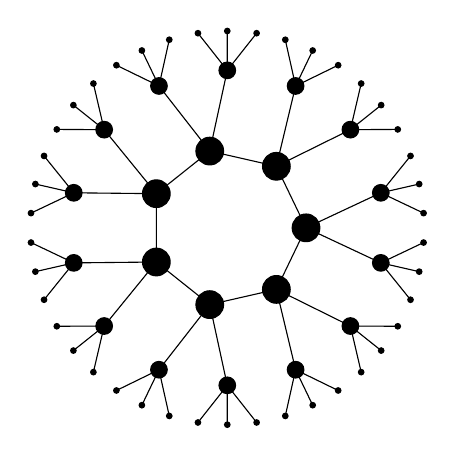
\begin{tikzpicture}
        \begin{scope}
          \def\crater{7}
          \foreach \i in {1,...,\crater} {
            \draw[fill] (360/\crater*\i:1cm) circle (5pt);
            \draw (360/\crater*\i : 1cm) -- (360/\crater*\i+360/\crater : 1cm);
            \foreach \j in {-1,1} {
              \draw[fill] (360/\crater*\i : 1cm) -- (360/\crater*\i + \j*360/\crater/4 : 2cm) circle (3pt);
              \foreach \k in {-1,0,1} {
                \draw[fill] (360/\crater*\i + \j*360/\crater/4 : 2cm) --
                (360/\crater*\i + + \j*360/\crater/4 + \k*360/\crater/6 : 2.5cm) circle (1pt);
              }
            }
          }
        \end{scope}
      \end{tikzpicture}
    \end{column}
  \end{columns}
\end{frame}

%%

\begin{frame}{Volcanology I}

  \begin{columns}
    \begin{column}{0.5\textwidth}
      Let $E,E'$ be curves with respective endomorphism rings $\O,\O'$.\\
      Let $\phi:E\to E'$ be an isogeny of prime degree $\ell$, then:
    \end{column}
    \begin{column}{0.5\textwidth}
      \centering{}
      \begin{tabular}{l l}
        if $\O=\O'$, & $\phi$ is \emph{horizontal};\\
        if $[\O':\O]=\ell$, & $\phi$ is \emph{ascending};\\
        if $[\O:\O']=\ell$, & $\phi$ is \emph{descending}.
      \end{tabular}      
    \end{column}
  \end{columns}

  \bigskip

  \centering
  \begin{tikzpicture}
    \def\crater{7}
    \foreach \i in {1,...,\crater} {
      \draw[fill] (360/\crater*\i:1cm) circle (5pt);
      \draw (360/\crater*\i : 1cm) -- (360/\crater*\i+360/\crater : 1cm);
      \foreach \j in {-1,1} {
        \draw[fill] (360/\crater*\i : 1cm) -- (360/\crater*\i + \j*360/\crater/4 : 2cm) circle (3pt);
        \foreach \k in {-1,0,1} {
          \draw[fill] (360/\crater*\i + \j*360/\crater/4 : 2cm) --
          (360/\crater*\i + + \j*360/\crater/4 + \k*360/\crater/6 : 2.5cm) circle (1pt);
        }
      }
    }
    \begin{scope}[xshift=4cm]
      \node at (0,2) {$\End(E)$};
      \draw[fill] (0,1) circle(5pt) node[xshift=0.7cm]{$\O_K$} -- 
      (0,0) circle(3pt) --
      (0,-1) circle(1pt) node[xshift=0.7cm]{$\Z[\pi]$};
    \end{scope}
  \end{tikzpicture}
  
  \small
  Isogeny volcano of degree $\ell=3$.
\end{frame}

%%

\begin{frame}{Volcanology II}
  \centering
  \begin{columns}
    \begin{column}{0.35\textwidth}
      \uncover<2->{Height $= v_\ell([\O_K:\Z[\pi]])$.}
      
      \bigskip
      
      \uncover<3->{\alert{How large is the crater?}}
    \end{column}
    \begin{column}{0.65\textwidth}
      \centering
      \begin{tikzpicture}[scale=0.9]
        \begin{scope}
          \def\crater{7}
          \foreach \i in {1,...,\crater} {
            \draw[fill] (360/\crater*\i:1cm) circle (5pt);
            \draw (360/\crater*\i : 1cm) -- (360/\crater*\i+360/\crater : 1cm);
            \foreach \j in {-1,1} {
              \draw[fill] (360/\crater*\i : 1cm) -- (360/\crater*\i + \j*360/\crater/4 : 2cm) circle (3pt);
              \foreach \k in {-1,0,1} {
                \draw[fill] (360/\crater*\i + \j*360/\crater/4 : 2cm) --
                (360/\crater*\i + + \j*360/\crater/4 + \k*360/\crater/6 : 2.5cm) circle (1pt);
              }
            }
          }
        \end{scope}
        \begin{scope}[xshift=4cm]
          \node at (0,2) {$\End(E)$};
          \draw[fill] (0,1) circle(5pt) node[xshift=0.7cm]{$\O_K$} -- 
          (0,0) circle(3pt) --
          (0,-1) circle(1pt) node[xshift=0.7cm]{$\Z[\pi]$};
        \end{scope}
      \end{tikzpicture}
    \end{column}  
  \end{columns}
  
  \bigskip
  
  \begin{tabular}{c | c | c c c}
    && \textbf{Horizontal} & \textbf{Ascending} & \textbf{Descending}\\
    \hline
    $\ell\nmid[\O_K:\O]]$ & $\ell\nmid[\O:\Z[\pi]]$ &$1+\left(\frac{D_K}{\ell}\right)$& &\\
    $\ell\nmid[\O_K:\O]]$ & $\ell\mid[\O:\Z[\pi]]$ &$1+\left(\frac{D_K}{\ell}\right)$& &$\ell-\left(\frac{D_K}{\ell}\right)$\\
    $\ell\mid[\O_K:\O]]$ & $\ell\mid[\O:\Z[\pi]]$ &  &$1$&$\ell$\\
    $\ell\mid[\O_K:\O]]$ & $\ell\nmid[\O:\Z[\pi]]$ & &$1$& 
  \end{tabular}
\end{frame}

%%

\begin{frame}{The class group}
  
  Let \emph{$\End(E) = \O \subset \Q(\sqrt{-D})$}. Define

  \begin{itemize}
  \item $\mathcal{I}(\O)$, the group of \emph{invertible fractional ideals},
  \item $\mathcal{P}(\O)$, the group of \emph{principal ideals},
  \end{itemize}
  
  \begin{block}{The class group}
    The \emph{class group} of $\O$ is
    \[\Cl(\O) = \mathcal{I}(\O)/\mathcal{P}(O).\]
  \end{block}

  \begin{itemize}
  \item It is a \emph{finite abelian} group.
  \item Its order \emph{$h(\O)$} is called the \emph{class number} of
    $\O$.
  \item It arises as the Galois group of an abelian extension of
    $\Q(\sqrt{-D})$.
  \end{itemize}
\end{frame}

%%

\begin{frame}
  \frametitle{Complex multiplication}
  
  \begin{block}{The $\a$-torsion}
    \begin{itemize}
    \item Let \emph{$\a\subset\O$} be an (integral invertible) ideal of
      $\O$;
    \item Let \emph{$E[\a]$} be the subgroup of $E$ annihilated by
      $\a$:
      \vspace{-2mm}
      \[E[\a] = \{P\in E \;|\; \alpha(P) = 0 \text{ for all } \alpha\in\a\};\]
    \item \vspace{-1mm} Let \emph{$\phi:E\to E_\a$}, where
      $E_\a=E/E[\a]$.
    \end{itemize}
    Then $\End(E_\a) = \O$ (i.e., $\phi$ is \emph{horizontal}).
  \end{block}


  \begin{theorem}[Complex multiplication]
    The action on the set of elliptic curves with complex
    multiplication by $\O$ defined by \emph{$\a\ast j(E) = j(E_\a)$}
    factors through $\Cl(\O)$, is faithful and transitive.
  \end{theorem}

  \begin{corollary}
    Let $\End(E)$ have discriminant $D$. Assume that
    $\left(\frac{D}{\ell}\right)=1$, then $E$ is on a crater of an
    $\ell$-volcano, and the crater contains $h(\End(E))$ curves.
  \end{corollary}
\end{frame}

%%

\begin{frame}{Supersingular graphs}
  \begin{columns}
    \begin{column}{0.6\textwidth}
      \begin{itemize}
      \item Every supersingular curve is defined over \emph{$\F_{p^2}$}.
      \item For every \emph{maximal order type} of the quaternion
        algebra $\Q_{p,\infty}$ there are \emph{$1$ or $2$ curves over
          $\F_{p^2}$} having endomorphism ring isomorphic to it.
      \item There is a \emph{unique isogeny class} of supersingular
        curves over $\bar{\F}_p$ of size \emph{$\sim p/12$}.
      \item Left ideals act on the set of maximal orders like isogenies.
      \item The graph of \emph{$\ell$}-isogenies is
        \emph{$(\ell+1)$}-regular.
      \end{itemize}
    \end{column}
    \begin{column}{0.4\textwidth}
      \centering
      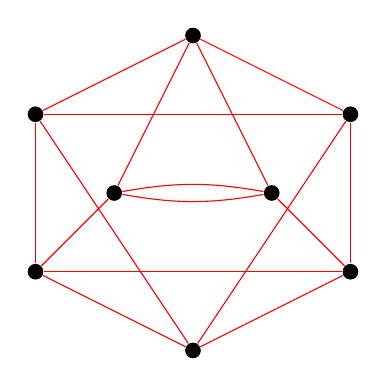
\begin{tikzpicture}
        \begin{scope}[every node/.style={fill,black,circle,inner sep=2pt}]
          \node at (0,0)  (1){};
          \node at (0,4) (20){};
          \node at (2,1)  (16z){};
          \node at (-2,1)  (81z){};
          \node at (-1,2) (77z){};
          \node at (1,2)  (20z){};
          \node at (-2,3)  (85z){};
          \node at (2,3)  (12z){};
        \end{scope}

        \begin{scope}[red]
          \path (1) edge (85z) edge (81z) edge (12z) edge (16z);
          \path (20) edge (85z) edge (77z) edge (20z) edge (12z);
          \path (81z) edge (85z) edge (77z) edge (16z);
          \path (85z) edge (12z);
          \path (12z) edge (16z);
          \path (16z) edge (20z);
          \path (20z) edge[bend right=10] (77z) edge[bend left=10] (77z);
        \end{scope}
      \end{tikzpicture}
      \small
      \emph{Figure:} $3$-isogeny graph on $\F_{97^2}$.
    \end{column}
  \end{columns}
\end{frame}

%%
%% 

\section{Isogeny-based cryptography}

\begin{frame}
  \frametitle{Overview}
  \tableofcontents  
\end{frame}

%%

\begin{frame}{Isogeny graphs}
  \begin{itemize}
  \item \emph{Vertices are curves} up to isomorphism,
  \item \emph{Edges are isogenies} up to isomorphism.
  \end{itemize}

  \begin{block}{Ordinary case}
    \begin{itemize}
    \item $\ell$-isogeny graphs form \emph{volcanoes}.
    \item The height of the volcano is given by the conductor of
      $\Z[\pi]$.
    \item All curves on the same level have the same endomorphism ring
      (have \emph{complex multiplication} by the same order $\O$).
    \item Type of summit (one curve, two curves, crater) determined by
      $\left(\frac{D}{\ell}\right)$.
    \item Size of the crater is $h(\O)$, and $\Cl(\O)$ acts on it.
    \end{itemize}
  \end{block}

  \begin{block}{Supersingular case}
    \begin{itemize}
    \item There are $\sim p/12$ supersingular $j$-invariants, all
      defined over $\F_{p^2}$.
    \item $\ell$-isogeny graphs are \emph{$(\ell+1)$-regular and
        connected}.
    \end{itemize}
  \end{block}
\end{frame}

%%

\subsection{Isogeny walks}

\begin{frame}{Graphs lexicon}
  \begin{description}
  \item[Degree:] Number of (outgoing/ingoing) edges.
  \item[$k$-regular:] All vertices have degree $k$.
  \item[Connected:] There is a path between any two vertices.
  \item[Distance:] The length of the shortest path between two vertices.
  \item[Diamater:] The longest distance between two vertices.
  \item[$\lambda_1\ge\cdots\ge\lambda_n$:] The (ordered) eigenvalues
    of the adjacency matrix.
  \end{description}
\end{frame}

%%

\begin{frame}{Expander graphs}
  \begin{block}{Proposition}
    If $G$ is a $k$-regular graph, its largest and smallest
    eigenvalues satisfy
    \[k = \lambda_1 \ge \lambda_n \ge -k.\]
  \end{block}
  
  \begin{block}{Expander families}
    An infinite family of connected $k$-regular graphs on $n$ vertices
    is an \emph{expander family} if there exists an $\epsilon>0$ such
    that all \emph{non-trivial} eigenvalues satisfy
    $|\lambda| \le (1-\epsilon)k$ for $n$ large enough.
  \end{block}
  
  \begin{itemize}
  \item Expander graphs have \emph{short diameter} ($O(\log n)$);
  \item Random walks \emph{mix rapidly} (after $O(\log n)$ steps,
    the induced distribution on the vertices is close to uniform).
  \end{itemize}
\end{frame}

%%

\begin{frame}{Expander graphs from isogenies}
  \begin{block}{Theorem (\cite{pizer1,pizer2})}
    Let $\ell$ be fixed. The family of graphs of \emph{supersingular}
    curves over $\F_{p^2}$ with $\ell$-isogenies, as $p\to\infty$, is
    an expander family\footnote{Even better, it has the Ramanujan
      property.}.
  \end{block}
  
  In the \emph{ordinary} case, for all primes \emph{$\ell \nmid t^2-4q$}:
  \begin{itemize}
  \item 50\% of $\ell$-isogeny graphs are isolated
    points,\hfill$\left(\frac{D_K}{\ell}\right)=-1$
  \item 50\% of $\ell$-isogeny graphs are
    \emph{cycles}.\hfill$\left(\frac{D_K}{\ell}\right)=+1$
  \end{itemize}
  
  \begin{block}{Theorem (\cite{jao+miller+venkatesan09})}
    Let $\O\subset\Q[\sqrt{-D}]$ be an order in a quadratic imaginary
    field. The graphs of all curves over $\F_q$ with \emph{complex
      multiplication by $\O$}, with isogenies of prime degree
    bounded\footnote{May contain traces of GRH.} by
    $(\log q)^{2+\delta}$, are expanders.
  \end{block}
\end{frame}

%%

\begin{frame}
  \frametitle{Isogeny based cryptography is 20 years old!}

  \begin{description}
  \item<1->[1996] Couveignes suggests \emph{isogeny-based
      key-exchange} at a seminar in École Normale Supérieure;
  \item<1->[1997] He submits \emph{``Hard Homogeneous Spaces''} to
    Crypto;
  \item<2->[1997] His paper gets \alert{rejected};
  \item<3->[1997--2006] \dots Nothing happens for about 10 years.
  \end{description}

  \bigskip
  
  \begin{uncoverenv}<4->
    \begin{center}
      \large
      
      \emph{Ok. Let's move on to the next 10 years!}
    \end{center}
  \end{uncoverenv}
\end{frame}

%%

\begin{frame}{Isogeny problems}
  \begin{block}{Isogeny computation\hfill\uncover<2->{$\mathrm{poly}(\#G)$}}
    Given an elliptic curve $E$ with Frobenius endomorphism $\pi$, and
    a subgroup $G\subset E$ such that $\pi(G)=G$, compute the rational
    fractions and the image curve of the separable isogeny
    $\phi:E\to E/G$.
  \end{block}

  \begin{block}{Explicit isogeny\hfill\uncover<3->{$\mathrm{poly}(d)$}}
    Given two elliptic curves $E,E'$ over a finite field, isogenous of
    known degree $d$, find an isogeny $\phi:E\to E'$ of degree $d$.
  \end{block}

  \begin{block}{Isogeny walk\hfill\uncover<4->{\alert{$\exp(\log\#k)$}}}
    Given two elliptic curves $E,E'$ over a finite field $k$, such
    that $\#E=\#E'$, find an isogeny $\phi:E\to E'$ of smooth degree.
  \end{block}
\end{frame}

%%

\begin{frame}
  \frametitle{Isogeny walks and
    cryptanalysis\footcite{galbraith99,GHS,bisson+sutherland11-rho} (circa 2000)}
  
  \emph{Fact:} Having a \emph{weak DLP} is not (always) isogeny invariant.

  \begin{center}
    \begin{tikzpicture}
      \path (0,0) node[anchor=east] {$E$} (6,0) node[anchor=west] {$E'$};
      \path[gray] (-0.8,0) node[anchor=east] {weak curve}
      (6.8,0) node[anchor=west] {strong curve};

      \draw[->] (0,0) -- (0.5,-0.2);
      \draw[->] (6,0) -- (5.5,0.2);
      \draw[->] (0.5,-0.2) -- (1,0.2);
      \draw[->] (5.5,0.2) -- (5,-0.2);
      \begin{scope}[densely dotted,coils/.style={decorate,decoration={coil,aspect=0,amplitude=2pt}}]
        \draw[coils] (1,0.2) -- (3,0.4);
        \draw[coils] (5,-0.2) -- (3,0.4);
        \draw[-angle 90,coils] (3,0.4) -- (3, -0.4) node[anchor=north] {$E''$};
      \end{scope}
    \end{tikzpicture}
  \end{center}
  
  \begin{block}{Fourth root attacks}
    \begin{itemize}
    \item Start two random walks from the two curves and wait for a
      collision.
    \item Over \emph{$\F_q$}, the average size of an isogeny class is
      \emph{$h(\O_K)\sim\sqrt{q}$}.
    \item A collision is expected after
      \emph{$O(\sqrt{h(\O_K)}) = O(q^{\frac{1}{4}})$} steps.
    \end{itemize}
  \end{block}

  \emph{Note:} Can be used to build \emph{trapdoor
    systems}\footcite{teske06}.

\end{frame}

%% 

\begin{frame}
  \frametitle{Random walks and hash functions (circa 2006)}

  Any expander graph gives rise to a hash function.

  \begin{center}
    \begin{tikzpicture}
      \coordinate (last) at (0,0);
      \draw (last) node[anchor=east] {$v$};
      \foreach \i in {1,...,6} {
        \pgfmathparse{(-1)^\i}
        \let\sign\pgfmathresult
        \pgfmathparse{int(mod(\i+1,2))}
        \let\bit\pgfmathresult
        \pgfmathparse{int(mod(\i,2))}
        \let\nbit\pgfmathresult
        \draw[->] (last) -- (\i,\sign*0.1) node[blue,pos=0.5,yshift=\sign*0.2cm]{\small$\bit$};
        \draw[dashed,->] (last) -- (\i,-\sign*0.5) node[gray,pos=0.5,yshift=-\sign*0.2cm]{\small$\nbit$};
        \coordinate (last) at (\i,\sign*0.1);
      }
      \draw (last) node[anchor=west] {$v'$};

      \node[blue,anchor=west] at (7,0) {$H(010101)=v'$};
    \end{tikzpicture}
  \end{center}

  \begin{itemize}
  \item Fix a starting vertex \emph{$v$};
  \item The value to be hashed determines a random path to \emph{$v'$};
  \item \emph{$v'$} is the hash.
  \end{itemize}

  \begin{block}{Provably secure hash functions}
    \begin{itemize}
    \item Use the expander graph of \alert{supersingular
        $2$-isogenies};\footcite{charles+lauter+goren09,doliskani+barreto+hash}
    \item \alert{Collision resistance} = hardness of finding cycles in the graph;
    \item \alert{Preimage resistance} = hardness of finding a path
      from \emph{$v$} to \emph{$v'$}.
    \end{itemize}
  \end{block}
\end{frame}

%%
%%

\subsection{Key exchange from ordinary graphs}

\begin{frame}
  \frametitle{Random walks and key exchange}

  \begin{flushleft}
    \Large
    Let's try something harder...
  \end{flushleft}

  \begin{center}
    \begin{tikzpicture}[xscale=0.7,yscale=0.4]
      \foreach \p/\psym/\psign in {Alice/A/-1,Bob/B/1} {
        \coordinate (last) at (\psign,0);
        \foreach \round in {0,1} {
          \pgfmathparse{\psign*(2*\round-1)}
          \let\rsign\pgfmathresult
          \foreach \i in {1,...,5} {
            \pgfmathparse{int(mod(mod(\i,2+(1+\psign)*0.5+\round),2))}
            \let\bit\pgfmathresult
            \pgfmathparse{int(mod(\bit+1,2))}
            \let\nbit\pgfmathresult
            \pgfmathparse{(-1)^(\bit)}
            \let\sign\pgfmathresult
            \draw[->] (last) -- ++(-\rsign,-1+\sign*0.1) node[blue,pos=0.5,yshift=\sign*0.1cm,xshift=-\sign*0.1cm*\rsign]{\small$\bit$};
            \draw[dashed,->,white!80!black] (last) -- ++(-\rsign+\sign*0.5*\rsign,-1-\sign*0.5) node[pos=0.5,yshift=-\sign*0.1cm,xshift=\sign*0.1cm*\rsign]{\small$\nbit$};
            \coordinate (last) at (-\i*\rsign+\round*5*\rsign+\psign,-\i-\round*6.6+\sign*0.1);
          }
          \coordinate (last) at (-5*\rsign+\psign,-6.6);
        }
      }
      \draw[alert] (0,0) node[anchor=south] {Public $v_0$}
      (-5,-5.2) node[anchor=north] {Alice's public $v_A$}
      (5,-5.2) node[anchor=north] {Bob's public $v_B$}
      (0,-11.8) node[anchor=north] {Shared secret};
    \end{tikzpicture}
  \end{center}

  \vspace{-1cm}
  
  \begin{flushright}
    \Large
    ...is this even possible?
  \end{flushright}
\end{frame}

%%

\begin{frame}
  \frametitle{Expander graphs from groups}
  \begin{center}
    \begin{tikzpicture}
      \begin{scope}
        \def\crater{12}
        \def\jumpa{-8}
        \def\jumpb{9}
        \def\diam{3cm}

        \foreach \i in {1,...,\crater} {
          \uncover<2->{\draw[blue] (360/\crater*\i : \diam) to[bend right] (360/\crater*\i+360/\crater : \diam);}
          \uncover<3->{\draw[red] (360/\crater*\i : \diam) to[bend right] (360/\crater*\i+\jumpa*360/\crater : \diam);}
          \uncover<4->{\draw[green] (360/\crater*\i : \diam) to[bend right=50] (360/\crater*\i+\jumpb*360/\crater : \diam);}
        }
        \foreach \i in {1,...,\crater} {
          \pgfmathparse{int(mod(2^\i,13))}
          \let\exp\pgfmathresult
          \draw[fill] (360/\crater*\i: \diam) circle (2pt) +(360/\crater*\i: 0.4) node{$g^{\exp}$};
        }
      \end{scope}
      \begin{scope}[xshift=4cm]
        \draw (0,2.1) node[anchor=west] {\parbox{4cm}{
            Let \emph{$G=\langle g\rangle$} be a cyclic group of order \emph{$p$}.
            \uncover<5->{Let \emph{$S\subset(\Z/p\Z)^\times$} s.t. \emph{$S^{-1}\subset S$}.\\
              The \emph{Schreier graph} of \emph{$(S,G\setminus\{1\})$} is (usually) an expander.}}};
        \uncover<2->{\draw[blue] (0,0) -- (0.5,0) (0.5,0) node[anchor=west] {$x \mapsto x^{2}$};}
        \uncover<3->{\draw[red] (0,-1) -- (0.5,-1) (0.5,-1) node[anchor=west] {$x \mapsto x^{3}$};}
        \uncover<4->{\draw[green] (0,-2) -- (0.5,-2) (0.5,-2) node[anchor=west] {$x \mapsto x^{5}$};}
      \end{scope}
    \end{tikzpicture}
  \end{center}
\end{frame}

%% 

{
  \newcommand{\myedge}[3]{
    \draw[#3] (360/\crater*#1 : \diam) to[bend right] (360/\crater*#2 : \diam);
  }

\begin{frame}
  \frametitle{Key exchange from Schreier graphs}

  \begin{columns}
    \begin{column}{0.55\textwidth}
      \begin{tikzpicture}
        \begin{scope}
          \def\crater{12}
          \def\jumpa{-8}
          \def\jumpb{9}
          \def\diam{2.5cm}
          
          \foreach \i in {1,...,\crater} {
            \pgfmathparse{int(mod(2^\i,13))}
            \let\exp\pgfmathresult
            \draw[fill] (360/\crater*\i: \diam) circle (2pt);
          }
          \uncover<2,6->{
            % Alice 1
            \myedge{0}{1}{blue}\myedge{1}{5}{red}\myedge{5}{6}{blue}\myedge{6}{3}{green}
          }
          \uncover<3,5>{
            % Bob 1
            \begin{scope}[dashed,thick]
              \myedge{0}{4}{red}\myedge{4}{8}{red}\myedge{8}{5}{green}\myedge{5}{6}{blue}
            \end{scope}
          }
          \uncover<5>{
            % Alice 2
            \myedge{6}{7}{blue}\myedge{7}{11}{red}\myedge{11}{0}{blue}\myedge{0}{9}{green}
          }
          \uncover<6->{
            % Bob 2
            \begin{scope}[dashed,thick]
              \myedge{3}{7}{red}\myedge{7}{11}{red}\myedge{11}{8}{green}\myedge{8}{9}{blue}
            \end{scope}
          }

          \draw (0 : \diam + 0.4cm) node {$g$};
          \uncover<2->{\draw (360/\crater*3 : \diam + 0.4cm) node {$g_A$};}
          \uncover<3->{\draw (360/\crater*6 : \diam + 0.4cm) node {$g_B$};}
          \uncover<5->{\draw (360/\crater*9 : \diam + 0.4cm) node {$g_{BA}\uncover<6->{=g_{AB}}$};}
        \end{scope}
      \end{tikzpicture}  
    \end{column}    
    \begin{column}{0.45\textwidth}
      \begin{onlyenv}<-6>
        \textbf{Public parameters:}
        \begin{itemize}
        \item A group \emph{$G=\langle g\rangle$} of order \emph{$p$};
        \item A subset \emph{$S\subset(\Z/p\Z)^\times$}.
        \end{itemize}
        \begin{enumerate}
        \item<2-> \textbf{Alice} takes a \alert{secret} random walk
          \emph{$s_A:g\to g_A$} of length \emph{$O(\log p)$};
        \item<3-> \textbf{Bob} does the same;
        \item<4-> They publish \emph{$g_A$} and \emph{$g_B$};
        \item<5-> \textbf{Alice} repeats her secret walk \emph{$s_A$}
          starting from \emph{$g_B$}.
        \item<6-> \textbf{Bob} repeats his secret walk \emph{$s_B$}
          starting from \emph{$g_A$}.
        \end{enumerate}
      \end{onlyenv}
      \begin{onlyenv}<7->
        \textbf{Why does this work?}
        \begin{align*}
          g_A &= g^{\bl{2}\cdot\rd{3}\cdot\bl{2}\cdot\gr{5}},\\
          g_B &= g^{\rd{3^2}\cdot\gr{5}\cdot\bl{2}},\\
          g_{BA} &= g_{AB} = g^{\bl{2^3}\cdot\rd{3^3}\cdot\gr{5^2}};
        \end{align*}
        and $g_A,g_B,g_{AB}$ are uniformly distributed in $G$\dots

        \bigskip
        
        \begin{uncoverenv}<8->
          \dots Indeed, this is just a twisted presentation of the
          \alert{classical Diffie-Hellman protocol!}
        \end{uncoverenv}
      \end{onlyenv}
    \end{column}
  \end{columns}
\end{frame}
}

%%

\begin{frame}
  \frametitle{Group action on isogeny graphs}

  \begin{columns}
    \begin{column}{0.5\textwidth}
      \centering
      \begin{tikzpicture}
        \begin{scope}
          \def\crater{11}
          \def\jump{5}
          \def\diam{2.5cm}

          \foreach \i in {1,...,\crater} {
            \draw[blue] (360/\crater*\i : \diam) to[bend right] (360/\crater*\i+360/\crater : \diam);
            \draw[red] (360/\crater*\i : \diam) to[bend left] (360/\crater*\i+\jump*360/\crater : \diam);
          }
          \foreach \i in {1,...,\crater}
          \draw[fill] (360/\crater*\i: \diam) circle (2pt);
        \end{scope}
        \begin{scope}[xshift=-1.5cm, yshift=-3.2cm]
          \draw[blue] (0,0) -- (0.5,0) (0.5,0) node[anchor=west] {\bl{$\ell_1$}-isogenies};
          \draw[red] (0,-1) -- (0.5,-1) (0.5,-1) node[anchor=west] {\rd{$\ell_2$}-isogenies};
        \end{scope}
      \end{tikzpicture}
    \end{column}
    \begin{column}{0.5\textwidth}
      \begin{itemize}
      \item There is a group action of the \emph{ideal class group}
        $\Cl(\O)$ on the set of ordinary curves with \emph{complex
          multiplication} by $\O$.
      \item Its Schreier graph is an isogeny graph (and an
        expander if we take enough generators)
      \end{itemize}
    \end{column}
  \end{columns}
\end{frame}

%%

\begin{frame}
  \frametitle{Key exchange in graphs of ordinary isogenies\footcite{Couv,R&S} (circa 2006)}
  
  \emph{Parameters:}
  \begin{itemize}
  \item \alert{$E/\F_p$ ordinary elliptic curve} with \textit{Frobenius
      endomorphism} $\pi$,
  \item primes \bl{$\ell_1$},\rd{$\ell_2$},\dots\
    such that $\left(\frac{D_\pi}{\ell_i}\right)=1$.
  \item A \textit{direction} for each $\ell_i$ (i.e.\ a choice of a root of
    $\pi^2-t\pi+q\mod\ell$).
  \end{itemize}

  \emph{Secret data:} \alert{Random walks} $\a,\b\in\Cl(\O)$ in the
  isogeny graph.
  
  \begin{center}
    \begin{tikzpicture}
      \Large
      \node[matrix of math nodes, ampersand replacement=\&, column sep=0cm, row sep=1cm] (diagram) {
        \& |(1)| E \\
        |(a)| \a\ast E \& \& |(b)| \b\ast E\\
        \& |(ab)| \a\b\ast E = \b\a\ast E\\
      };
      \small
      \path[->] (1) edge node[auto,swap]{$\bl{\ell_1^{a_1}}\rd{\ell_2^{a_2}}\cdots=\mathcal{N}(\a)$} (a);
      \path[->] (1) edge node[auto]{$\mathcal{N}(\b)=\bl{\ell_1^{b_1}}\rd{\ell_2^{b_2}}\cdots$} (b);
      \path[->] (a) edge (ab);
      \path[->] (b) edge (ab);
    \end{tikzpicture}
  \end{center}
\end{frame}

%%

\begin{frame}{CRS key exchange}

  \begin{center}
    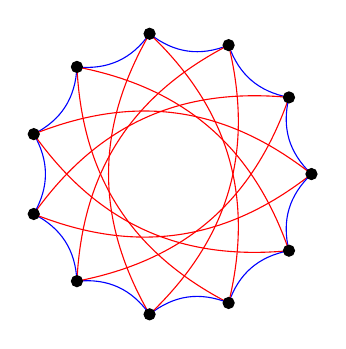
\begin{tikzpicture}
      \begin{scope}
        \def\crater{11}
        \def\jump{5}
        \def\diam{1.8cm}

        \foreach \i in {1,...,\crater} {
          \draw[blue] (360/\crater*\i : \diam) to[bend left] (360/\crater*\i+360/\crater : \diam);
          \draw[red] (360/\crater*\i : \diam) to[bend right] (360/\crater*\i+\jump*360/\crater : \diam);
        }
        \foreach \i in {1,...,\crater}
          \draw[fill] (360/\crater*\i: \diam) circle (2pt);
      \end{scope}
    \end{tikzpicture}
  \end{center}

  \begin{description}
  \item[Key generation:] compose small degree isogenies\\
    (Isogeny Computation Problem)\\
    \alert{polynomial in the length of the random walk}.
  \item[Attack:] Isogeny Walk Problem\\
    \alert{polynomial in the degree, exponential in the length}.
  \item[Open problem:] Make this thing practical!
  \end{description}
\end{frame}

%%

\begin{frame}{Security of CRS}
  \begin{description}
  \item[Size of the graph:] $h(\O)\sim\sqrt{p}$,
  \item[Key space size:] Exponential in the number of primes
    \bl{$\ell_1$},\rd{$\ell_2$},\dots\
  \item[Meet in the middle attack:] $O(\sqrt[4]{p})$.
  \end{description}

  \begin{block}{The Abelian Hidden Shift Problem}
    Let $G$ be a group and $S$ be a set. Given two oracles
    $f_0,f_1:G\to S$ such that \emph{$f_0(g)=f_1(gs)$} for some
    $s\in G$, \emph{find $s$}.
  \end{block}

  \begin{block}{Ordinary isogeny walk $\to$ Hidden shift}
    To find a secret isogeny walk $E_0\to E_1$, set
    \begin{align*}
      f_0 : \Cl(\O) &\to V & f_1 : \Cl(\O) &\to V\\
      \a &\mapsto \a\ast E_0 & \a &\mapsto \a\ast E_1
    \end{align*}
    Then the hidden shift is \emph{$\mathfrak{s}$} such that
    \emph{$\mathfrak{s}\ast E_0 = E_1$}.
  \end{block}
\end{frame}

%%

\begin{frame}
  \frametitle{Quantum attack on CRS\footcite{childs+jao+soukharev10}}

  \begin{enumerate}
  \item \alert{$L_p(1/2,\sqrt{3}/2)$} classical algorithm for
    evaluating $f_0,f_1$.
  \item Hidden Shift Problem $\to$ Dihedral Hidden
    Subgroup Problem.
  \end{enumerate}
  
  \begin{block}{Quantum algorithms for dihedral HSP}
    \begin{description}
    \item[Kuperberg\footcite{Kup}:] \alert{$2^{O(\sqrt{\log|G|})}$}
      quantum time, space and query complexity.
    \item[Regev\footcite{regev04}:]
      \alert{$L_{|G|}(\frac{1}{2},\sqrt{2})$} quantum time and query
      complexity, \alert{$\text{poly}(\log(|G|)$} quantum space.
    \end{description}
  \end{block}
\end{frame}

%%
%%

\subsection{Key exchange from supersingular graphs}

\begin{frame}
  \frametitle{Key exchange with supersingular curves (2011)}
  
  \begin{description}
  \item[Good news:] there is no action of a commutative class group.
  \item[Bad news:] there is no action of a commutative class group.
  \item[Idea:] Let \bl{Alice} and \rd{Bob} walk in two
    \emph{different isogeny graphs} on the \emph{same vertex set}.
  \end{description}

  \begin{columns}
    \begin{column}{0.7\textwidth}
      \centering
      \begin{tikzpicture}[scale=1.4]
        \begin{scope}[every node/.style={fill,black,circle,inner sep=2pt}]
          \node at (0,0)  (1){};
          \node at (0,4) (20){};
          \node at (2,1)  (16z){};
          \node at (-2,1)  (81z){};
          \node at (-1,2) (77z){};
          \node at (1,2)  (20z){};
          \node at (-2,3)  (85z){};
          \node at (2,3)  (12z){};
        \end{scope}

        \begin{uncoverenv}<1,3>
          \begin{scope}[blue,every loop/.style={looseness=50}]
            \path (1) edge (20) edge (16z) edge (81z);
            \path (20) edge[loop left] (20) edge[loop right] (20);
            \path (16z) edge (81z) edge (77z);
            \path (81z) edge (20z);
            \path (77z) edge (20z) edge (85z);
            \path (20z) edge (12z);
            \path (12z) edge[bend right=10] (85z) edge[bend left=10] (85z);
          \end{scope}
        \end{uncoverenv}
        
        \begin{uncoverenv}<2->
          \begin{scope}[red]
            \path (1) edge (85z) edge (81z) edge (12z) edge (16z);
            \path (20) edge (85z) edge (77z) edge (20z) edge (12z);
            \path (81z) edge (85z) edge (77z) edge (16z);
            \path (85z) edge (12z);
            \path (12z) edge (16z);
            \path (16z) edge (20z);
            \path (20z) edge[bend right=10] (77z) edge[bend left=10] (77z);
          \end{scope}
        \end{uncoverenv}
      \end{tikzpicture}
    \end{column}
    \begin{column}{0.3\textwidth}
      \small
      \emph{Figure:} \bl{$2$}- and \rd{$3$}-isogeny graphs on $\F_{97^2}$.
    \end{column}
  \end{columns}
\end{frame}

%%

\begin{frame}
  \frametitle{Key exchange with supersingular curves}

  \begin{itemize}
  \item Fix small primes \bl{$\ell_A$}, \rd{$\ell_B$};
  \item \emph{No canonical labeling} of the \bl{$\ell_A$}- and
    \rd{$\ell_B$}-isogeny graphs; \emph{however\dots}
  \end{itemize}

  \begin{center}
    \bf
    Walk of length \bl{$e_A$}\\
    $=$\\
    Isogeny of degree \bl{$\ell_A^{e_A}$}\\
    $=$\\
    Kernel \bl{$\langle P\rangle\subset E[\ell_A^{e_A}]$}
  \end{center}
  
  \begin{center}
    \begin{tikzpicture}
      \begin{scope}
        \draw (0,1.2) node[anchor=east,blue] {$\ker\phi=\cyc{P}\subset E[\ell_A^{e_A}]$};
        \draw (0,0.4) node[anchor=east,red] {$\ker\psi=\cyc{Q}\subset E[\ell_B^{e_B}]$};
        \draw (0,-0.4) node[anchor=east,blue] {$\ker\phi' = \cyc{\rd{\psi}(P)}$};
        \draw (0,-1.2) node[anchor=east,red] {$\ker\psi' = \cyc{\bl{\phi}(Q)}$};
      \end{scope}
      \begin{scope}[xshift=4.5cm,coils/.style={-angle 90,decorate,decoration={coil,aspect=0,amplitude=1pt}}]
        \large
        \node[matrix of nodes, ampersand replacement=\&, column sep=3cm, row sep=1.5cm] (diagram) {
          |(E)| $E$ \& |(Es)| $E/\cyc{\bl{P}}$ \\
          |(Ep)| {$E/\cyc{\rd{Q}}$} \& |(Eps)| {$E/\cyc{\bl{P},\rd{Q}}$}\\
        };
        \path[->,blue] (E) edge[coils] node[auto] {$\phi$} (Es);
        \path[->,blue] (Ep) edge[coils] node[auto,swap] {$\phi'$} (Eps);
        \path[->,red] (E) edge[coils] node[auto,swap] {$\psi$} (Ep);
        \path[->,red] (Es) edge[coils] node[auto] {$\psi'$} (Eps);
      \end{scope}
    \end{tikzpicture}
  \end{center}
\end{frame}

%%

\begin{frame}
  \frametitle{Supersingular Isogeny
    Diffie-Hellman\footcite{jao+defeo2011,defeo+jao+plut12}}

  \vspace{-1cm}

  \begin{columns}
    \begin{column}{0.4\textwidth}
      \begin{block}{}
        \emph{Parameters:}
        \begin{itemize}
          \setlength{\itemsep}{1.5ex}
        \item Prime $p$ such that $p+1 = \bl{\ell_A^a}\rd{\ell_B^b}$;
        \item Supersingular curve \emph{$E\simeq (\Z/(p+1)\Z)^2$};
        \item \bl{$E[\ell_A^a] = \cyc{P_A,Q_A}$};
        \item \rd{$E[\ell_B^b] = \cyc{P_B,Q_B}$}.
        \end{itemize}

        \emph{Secret data:}
        \begin{itemize}
          \setlength{\itemsep}{1.5ex}
        \item \bl{$R_A = m_AP_A + n_AQ_A$},
        \item \rd{$R_B = m_BP_B + n_BQ_B$},
        \end{itemize}
      \end{block}
    \end{column}
    \begin{column}{0.58\textwidth}
      \begin{center}
        \begin{tikzpicture}[coils/.style={-angle 90,decorate,decoration={coil,aspect=0,amplitude=1pt}}]
          \large
          \node[matrix of nodes, ampersand replacement=\&, column sep=4mm, row sep=2cm] (diagram) {
            \& |(1)| $E$ \\
            |(a)| \parbox{1.5cm}{$E/\cyc{\bl{R_A}}$\\\uncover<2->{{\footnotesize $\bl{\phi(}\rd{P_B}\bl{)}\\\bl{\phi(}\rd{Q_B}\bl{)}$}}} \& \&
            |(b)| \parbox{1.5cm}{$E/\cyc{\rd{R_B}}$\\\uncover<2->{{\footnotesize $\rd{\psi(}\bl{P_A}\rd{)}\\\rd{\psi(}\bl{Q_A}\rd{)}$}}}\\
            \normalsize $\frac{E/\cyc{\bl{R_A}}}{\alert{\bl{\phi(}\rd{R_B}\bl{)}}} \simeq$ \&
            |(ab)|  $E/\cyc{\bl{R_A},\rd{R_B}}$ \&
            \normalsize $\simeq \frac{E/\cyc{\rd{R_B}}}{\alert{\rd{\psi(}\bl{R_A}\rd{)}}}$\\
          };
          \small
          \path[blue] (1) edge[coils] node[auto,swap](phia) {$\phi$} (a);
          \path[red] (1) edge[coils] node[auto](phib) {$\psi$} (b);
          \path[red] (a) edge[coils] node[auto,swap](psia){$\psi'$} (ab);
          \path[blue] (b) edge[coils] node[auto](psib){$\phi'$} (ab);
          \uncover<3>{\path[dashed,->] (phia) edge node[auto]{\footnotesize $\bl{\phi(}\rd{R_B}\bl{)}$} (psia);}
          \uncover<3>{\path[dashed,->] (phib) edge node[auto,swap]{\footnotesize $\rd{\psi(}\bl{R_A}\rd{)}$} (psib);}
        \end{tikzpicture}
      \end{center}  
    \end{column}
  \end{columns}
\end{frame}

%% 

\begin{frame}
  \frametitle{Generic attacks}
  
  \emph{Problem:} Given \emph{$E,E'$}, isogenous of degree
  \emph{$\ell^n$}, find \emph{$\phi:E\to E'$}.

  \begin{center}
    \begin{tikzpicture}[xscale=4,coils/.style={-angle 90,decorate,decoration={coil,aspect=0,amplitude=1pt}}]
      \large
      \draw (0,2) node(E) {$E$};

      \draw (1,4) node(E1) {$E/\cyc{P_0}$};
      \draw (1,2) node(Ei) {$E_i/\cyc{P_i}$};
      \draw (1,0) node(En) {$E/\cyc{P_{\ell^{n/2}}}$};
      \draw (1,3) node(dots1) {$\vdots$};
      \draw (1,1) node(dots2) {$\vdots$};

      \draw (2,2) node(E') {$E'$};

      \draw (E) edge[coils] node[auto] {\normalsize$\ell^{n/2}$} (E1);
      \draw (E) edge[coils] (Ei);
      \draw (E) edge[coils] (En);
      \draw (E) edge[coils] (dots1);
      \draw (E) edge[coils] (dots2);

      \draw (E') edge[coils] node[auto,swap] {\normalsize$\ell^{n/2}$} (Ei);
    \end{tikzpicture}
  \end{center}

  \begin{itemize}
  \item With high probability $\phi$ is the unique collision (or
    \textit{claw}) $\alert{O(\ell^{n/2})}$.
  \item A \emph{quantum claw finding}\footcite{tani08} algorithm solves
    the problem in $\alert{O(\ell^{n/3})}$.
  \end{itemize}
\end{frame}

%%

\begin{frame}{Security}
  \begin{block}{The SIDH problem}
    Given \emph{$E$}, Alice's public data
    \emph{$E/\cyc{R_A}, \phi(P_B), \phi(Q_B)$}, and Bob's public data
    \emph{$E/\cyc{R_B}, \psi(P_A), \psi(Q_A)$}, find the shared secret
    \emph{$E/\cyc{R_A,R_B}$}.
  \end{block}

  Under the SIDH assumption:
  \begin{itemize}
  \item The SIDH key exchange protocol is \emph{session-key secure}.
  \item The derived El Gamal-type PKE is \emph{CPA secure}.
  \end{itemize}

  \begin{block}{Reductions}
    \begin{itemize}
    \item SIDH $\to$ Isogeny Walk Problem;
    \item SIDH $\to$ \emph{Computing the endomorphism rings} of $E$
      and
      $E/\cyc{R_A}$.\footcite{kohel2014quaternion,galbraithsecurity}
    \end{itemize}
  \end{block}
\end{frame}

%%

\begin{frame}{Chosen ciphertext attack\footcite{galbraithsecurity}}
  For simplicity, assume Alice's prime is $\ell = 2$.
  
  \begin{block}{Evil Bob}
    \begin{itemize}
    \item Alice has a long-term secret $\bl R = \bl mP + \bl nQ\in E[2^e]$;
    \item Bob produces an ephemeral secret $\rd\psi$;
    \item Bob sends to Alice $\rd\psi(P), \rd\psi(Q+2^{e-1}P)$;
    \item Alice computes the shared secret correctly iff
      \vspace{-2mm}
      \begin{align*}
        \bl R &= \bl mP + \bl nQ\\
        &= \bl mP + \bl nQ + \bl n2^{e-1}P,
      \end{align*}
      \vspace{-2mm}
      i.e., iff $\bl n$ is even;
    \item Bob \emph{learns one bit} of the secret key by checking that
      Alice gets the right shared secret.
    \end{itemize}
  \end{block}  

  \begin{itemize}
  \item Bob repeats the queries in a similar fashion, \emph{learning
      one bit per query}.
  \item Detecting Bob's faulty key seems to be as hard as breaking SIDH.
  \end{itemize}
\end{frame}

%%

\begin{frame}
  \frametitle{Bonus: a ZK proof of knowledge\footcite{defeo+jao+plut12}}
  
  \emph{Secret}: knowledge of the \emph{kernel} of a degree
  \bl{$\ell_A^{e_A}$} isogeny from $E$ to $E/\cyc{\bl{S}}$.
  \vspace{-2mm}
  \begin{center}
    \begin{tikzpicture}
      \large
      \node[matrix of nodes, ampersand replacement=\&, column sep=3cm, row sep=1.5cm] (diagram) {
        |(E)| $E$ \& |(Es)| $E/\cyc{\bl{S}}$ \\
        |(Ep)| {\uncover<2->{$E/\cyc{\rd{P}}$}} \& |(Eps)| {\uncover<2->{$E/\cyc{\rd{P},\bl{S}}$}}\\
      };
      \path[blue] (E) edge node[auto] {$\phi$} (Es);
      \uncover<2->{\path[blue] (Ep) edge node[auto,swap] {\alt<4->{$\phi'$}{\phantom{$\phi'$}?}} (Eps);}
      \uncover<2->{\path[red] (E) edge node[auto,swap] {\alt<3>{$\psi$}{?}} (Ep);}
      \uncover<2->{\path[red] (Eps) edge node[auto,swap] {\alt<3>{$\psi'$}{?}} (Es);}
    \end{tikzpicture}  
  \end{center}
  \vspace{-4mm}
  \begin{enumerate}
  \item<2-> Choose a random point \rd{$P\in E[\ell_B^{e_B}]$}, compute the diagram;
  \item<2-> Publish the curves $E/\cyc{\rd{P}}$ and $E/\cyc{\rd{P},\bl{S}}$;
  \item<3-> The verifier asks one of the two questions:
    \begin{itemize}
    \item<3-> Reveal the degree \rd{$\ell_B^{e_B}$} isogenies;
    \item<4-> Reveal the \bl{bottom} isogeny.
    \end{itemize}
  \end{enumerate}

  \uncover<5->{Can derive Fiat-Shamir \emph{signatures}: secure under
    SIDH\dots but very slow!}
\end{frame}  

%% 
%%

\subsection{The SIKE submission}

\begin{frame}{SIKE: Supersingular Isogeny Key Encapsulation}
  \begin{itemize}
  \item Submission to the \emph{NIST PQ competition}:
    \begin{description}
    \item[SIKE.PKE:] El Gamal-type system with \emph{IND-CPA} security
      proof,
    \item[SIKE.KEM:] generically transformed system with
      \emph{IND-CCA} security proof.
    \end{description}
  \item Security levels 1, 3 and 5.
  \item \emph{Smallest communication complexity} among all proposals
    in each level.
  \item \emph{Slowest} among all benchmarked proposals in each level.
  \item A team of 14 submitters, from 8 universities and companies.
  \item Download the package
    \href{https://csrc.nist.gov/CSRC/media/Projects/Post-Quantum-Cryptography/documents/round-1/submissions/SIKE.zip}{\emph{here}}.
  \end{itemize}

  \centering
  \begin{tabular}{l | c c c c c }
    & $p$ & cl. security & q. security & speed & comm.\\
    \hline
    SIKEp503 & $2^{250}3^{159}-1$ & 126 bits & 84 bits & 10ms & 0.4KB\\
    SIKEp751 & $2^{372}3^{239}-1$ & 188 bits & 125 bits & 30ms & 0.6KB\\
    SIKEp964 & $2^{486}3^{301}-1$ & 241 bits & 161 bits & & 0.8KB
  \end{tabular}
\end{frame}

%%

\begin{frame}{Parameter choices}
  \begin{description}
  \item[For efficiency:] $p = 2^a3^b - 1$, with $a$ even;
  \item[For security:]
    \[a \sim (\log_2 3) b \ge
      \begin{cases}
        2 \times \text{classical
          security parameter,}\\
        3 \times \text{quantum
          security parameter;}
      \end{cases}\]
  \item[For verifiability:] \
    \begin{itemize}
    \item Special starting curve $E_0 \;:\; y^2 = x^3 + x$;
    \item $P_A,Q_A,P_B,Q_B$ chosen as the lexicographically first
      points satisfying the necessary conditions.
    \end{itemize}
  \end{description}
\end{frame}

%%

\begin{frame}{Implementation: finite field}
  \begin{block}{Arithmetic in $\F_p$}
    \begin{itemize}
    \item $p = 2^a3^b - 1$ lends itself to optimizations:
      \begin{itemize}
      \item Adapted Comba-based Montgomery reduction\footcite{costello2016sidh},
      \item Adapted Barret reduction\footcite{vercauteren-sidh-fp};
      \item Assembly optimized.
      \end{itemize}
    \end{itemize}
  \end{block}

  \begin{block}{Arithmetic in $\F_{p^2}$}
    Because $p = -1 \mod 4$, then $-1$ is not a quadratic residue in
    $\F_p$. We define \emph{$\F_{p^2} = \F_p[i] = \F_p[X]/(X^2+1)$}.
    \begin{itemize}
    \item Arithmetic similar to $\Q[i]$;
    \item Karatsuba-like formulas for multiplication and squaring;
    \item Inversion only requires one inversion in $\F_p$;
    \item Optimizations similar to pairing-base crypto (e.g., BN254).
    \end{itemize}
  \end{block}
\end{frame}

%%

\begin{frame}{Implementation: curves}
  \begin{block}{Montgomery curves}
    Not a Weierstrass equation:
    \[\emph{b}y^2 = x^3 + \emph{a}x^2 + x\]
    \begin{itemize}
    \item Only possible for curves with a $4$-torsion point (we're
      lucky);
    \item Very efficient arithmetic in \emph{$XZ$-coordinates}:
      identify $\pm P$ by dropping the $Y$-coordinate
    \end{itemize}
  \end{block}

  Doubling:
  \[[2](X:\;\cdot\;:Z) = \bigl((X^2 - Z^2)^2:\;\cdot\;:4XZ(X^2+\emph{a}XZ+Z^2)\bigr)\]

  Tripling:
  \footnotesize
  \[[3](X:\;\cdot\;:Z) =
    \bigl(X(X^4-6X^2Z^2-4\emph{a}XZ^3-3Z^4):\;\cdot\;:Z(3X^4+4\emph{a}X^3Z+6X^2Z^3-Z^4)\bigr)\]
\end{frame}

%%

\begin{frame}{Implementation: curves}
  \begin{block}{Computing \emph{$mP + nQ$}}
    \begin{itemize}
    \item Observe that \emph{$mP +nQ$} and \emph{$P+(n/m)Q$} generate
      \emph{the same isogeny kernel};
    \item \emph{Constant time Montgomery ladder}
      tailored\footcite{cryptoeprint:2017:1015} to \emph{$P+cQ$}.
    \item For simplicity and \emph{constant-time sampling}, SIKE
      secret keys are restricted to \emph{$P+cQ$} with
      \emph{$c\in[0,\dots,2^x-1]$}.
    \end{itemize}
  \end{block}

  \begin{description}
  \item[Input] {\small $P=(X_P:Z_P), Q=(X_Q:Z_Q), P-Q=(X_{P-Q}:Z_{P-Q})$,\\
      a scalar $c$;}
  \item[Output] {\small $P+cQ$.}
  \end{description}
  \begin{enumerate}
  \item Set $R_0 = Q,\quad R_1= P,\quad R_2=Q-P$
  \item For $i$ from $0$ to $\lfloor\log_2 c\rfloor$:
    \begin{itemize}
    \item if $c_i = 0$, let $\quad R_0, R_1 \quad=\quad 2R_0,\;\; R_0+R_1$;
    \item if $c_i = 1$, let $\quad R_0, R_2 \quad=\quad 2R_0,\;\; R_0+R_2$;
    \end{itemize}
  \item Return $R_1$.
  \end{enumerate}
\end{frame}

%%

\begin{frame}{Implementation: isogenies}
  \begin{block}{Vélu's formulas}
    Given a group $G\subset E$, the isogeny $\phi:E\to E/G$ is defined by:
    \footnotesize
    \[\phi(P) = \left(x(P) + \sum_{Q\in G\setminus\{\O\}}x(P+Q) - x(Q),\right.
      \left.y(P) + \sum_{Q\in G\setminus\{\O\}}y(P+Q) - y(Q)\right).\]
  \end{block}
  
  \begin{block}{$3$-isogenies of Montgomery curves}
    Let $P = (X_3:Z_3)$ be a point of order $3$ on
    $\emph{b}y^2 = x^3 + \emph{a}x^2 + x$. The curve $E/\cyc{P}$ has
    equation $\emph{b}y^2 = x^3 + \emph{a'}x^2 + x$ where
    \[\emph{a'} = (\emph{a}X_3Z_3+6(Z_3^2-X_3^2))X_3\alert{/Z_3^3}.\]
    It is defined by the map
    \[\phi(X:Z) = \bigl(X(X_3X-Z_3Z)^2 \;:\; Z(Z_3X-X_3Z)^2\bigr).\]
  \end{block}

  Similar formula for \emph{$4$-isogenies}.
\end{frame}

%%

\begin{frame}{Implementation: isogeny walks}
  
  \emph{$\ord(R)=\ell^e$} and \emph{$\phi = \phi_0 \circ \phi_1 \circ \cdots
    \circ \phi_{e-1}$}, each of degree $\emph{\ell}$

  \begin{center}
  \begin{tikzpicture}[/triangle,scale=1.1]
    \def\n{5}
    \pgfmathtruncatemacro{\pn}{\n-1}
    

    \draw(-0.4,-0.2) node{$R$};

    \foreach \i in {1,...,\n} {
      \draw(\i,\i+0.7) node{$R_\i$};
    }
    \foreach \i in {1,...,\n} {
      \draw(\i,-1) node{$[\ell^\i]R$};
    }
    \foreach \i in {0,...,\pn} {
      \pgfmathtruncatemacro{\ii}{\pn-\i}
      \foreach \j in {0,...,\ii} {
        \draw(\i+\j+0.4,\i+0.6) node{$\phi_\i$};
      }
    }
    \foreach \i in {0,...,\pn} {
      \draw(\i+0.5,-0.2) node{$[\ell]$};
    }

    \foreach \i in {1,...,\pn} {
      \pgfmathtruncatemacro{\ii}{\n-\i}
      \draw(\n+0.5,1.15*\i-0.1) node{\emph{\small $[\ell^\ii]R_\i$}};
    }

    \foreach \i in {0,...,\pn} {
      \foreach \j in {0,...,\i} {
        \draw[gray,dashed]  (\i,\j) -- (\i+1,\j+1);
        \draw[gray,dashed]  (\i,\j) -- (\i+1,\j);
      }
    }

    \dottriangle[$\bullet$]{\n}
  \end{tikzpicture}
  \end{center}
  For each $i$, one needs to compute \emph{$[\ell^{e-i}]R_i$} in
  order to compute $\phi_i$.
\end{frame}

%%

\begin{frame}{Implementation: isogeny walks}

  \begin{figure}
    \centering
    \begin{tikzpicture}[/triangle,scale=0.35]
      \def\n{3}
      \newlength{\shift}
      \setlength{\shift}{5cm}

      \foreach \k in {0,...,6} {
        \begin{scope}[xshift=\k\shift]
          \dottriangle[$\cdot$]{\n}
          \foreach \i in {1,...,\n} {
            \draw(\i-1,0) -- (\i,0);
          }
          \foreach \i in {1,...,\n} {
            \draw(\i-1,\i-1) -- (\i,\i);
          }
        \end{scope}
      }

      \begin{scope}
        \draw (1,0)--(2,1) (2,1)--(3,2) (2,0)--(3,1);
      \end{scope}

      \begin{scope}[xshift=\shift]
        \draw (1,0)--(2,1) (2,1)--(3,1) (2,1)--(3,2);
      \end{scope}

      \begin{scope}[xshift=2\shift]
        \draw (1,0)--(2,1) (2,1)--(3,1) (2,2)--(3,2);
      \end{scope}

      \begin{scope}[xshift=3\shift]
        \draw (2,0)--(3,1) (2,2)--(3,2);
      \end{scope}

      \begin{scope}[xshift=4\shift]
        \draw (1,1)--(2,1) (2,1)--(3,2) (2,0)--(3,1);
      \end{scope}

      \begin{scope}[xshift=5\shift]
        \draw (1,1)--(2,1) (2,1)--(3,2) (2,1)--(3,1);
      \end{scope}

      \begin{scope}[xshift=6\shift]
        \draw (1,1)--(2,1) (2,1)--(3,1) (2,2)--(3,2);
      \end{scope}
    \end{tikzpicture}
    \caption{The seven well formed strategies for $e=4$.}
  \end{figure}

  \begin{itemize}
  \item Right edges are \emph{$\ell$-isogeny evaluation};
  \item Left edges are \emph{multiplications by $\ell$} (about twice as expensive);
  \item The best strategy can be \emph{precomputed} offline and
    \emph{hardcoded}.
  \item Evaluation is done in \emph{constant time}!
  \item Pre-computed optimized strategies are given in the SIKE
    submission document.
  \end{itemize}
\end{frame}

%% 

\begin{frame}{Example}
  \begin{figure}[t]
    \centering
    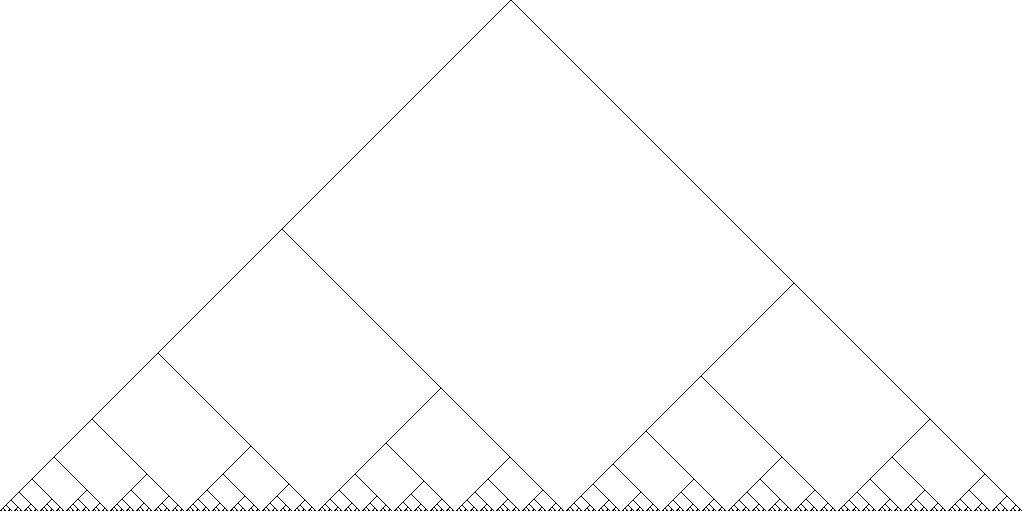
\includegraphics[width=\textwidth]{optimal.png}
    \caption{Optimal strategy for $e=512$, $\ell=2$.}
    \label{fig:optimal}
  \end{figure}
\end{frame}

%%

\begin{frame}{Implementation: constant time}
  \begin{itemize}
  \item Secret key sampling in constant time by \emph{restricting key
      space};
  \item $P + cQ$ in constant time via \emph{Montgomery ladder};
  \item Isogeny walk in constant time via \emph{any strategy}.
  \end{itemize}

  \begin{block}{Finite field operations in constant time}
    Only problem is to \emph{avoid inversions} as much as possible,
    but Vélu's formulas require one inversion per curve on the walk.

    \textbf{Solution\footcite{costello2016sidh}:} \emph{projectivize
      curve equations}
    \vspace{-4mm}
    \[E\;:\;\emph{CB}y^2 = \emph{C}x^3 + \emph{A}x^2 + \emph{C}x.\]
    \vspace{-0.9cm}
    \begin{itemize}
    \item Slightly increases operation counts of formulas;
    \item Delays all inversions to the very end;
    \item Only the value $(A:C)$ is needed in computations. Then:
      \[j(E) = \frac{256(A^2-3C^2)}{C^4(A^2-4C^2)}.\]
    \end{itemize}
  \end{block}
\end{frame}

%%

\begin{frame}{Summary}
  \emph{Public parameters:}
  \begin{itemize}
  \item $p = 2^a3^b - 1$,
  \item Staring curve $E\;:\; y^2 = x^3 + x$,
  \item Torsion generators
    \begin{gather*}
      P_A = (X_{a1}:Z_{a1}), \quad Q_A = (X_{a2}:Z_{a2}), \quad P_A-Q_A =  (X_{a3}:Z_{a3}),\\
      P_B = (X_{b1}:Z_{b1}), \quad Q_B = (X_{b2}:Z_{b2}), \quad P_B-Q_B =  (X_{b3}:Z_{b3}).
    \end{gather*}
  \end{itemize}

  \emph{Secret keys:}
  \begin{itemize}
  \item $R_A = P_A + cQ_A$ with $c\in[0,\dots,2^a-1]$,
  \item $R_B = P_A + cQ_A$ with $c\in[0,\dots,2^{b\lfloor\log_23\rfloor}-1]$.
  \end{itemize}

  \emph{Public keys (curve equation can be interpolated from three points):}
  \begin{itemize}
  \item $\phi(P_B), \phi(Q_B), \phi(P_B-Q_B)$,
  \item $\psi(P_A), \psi(Q_A), \psi(P_A-Q_A)$.
  \end{itemize}

  \emph{Shared secret:}
  \begin{itemize}
  \item $j = 256(A^2-3C^2)/C^4(A^2-4C^2)$.
  \end{itemize}
\end{frame}

%%
%% 

%%

\begin{frame}
  \centering
  \begin{tikzpicture}
    \begin{scope}[xscale=1.2,black!60]
      \def\crater{7}
      \foreach \i in {1,...,\crater} {
        \draw[fill] (360/\crater*\i:3cm) circle (5pt);
        \draw (360/\crater*\i : 3cm) -- (360/\crater*\i+360/\crater : 3cm);
        \foreach \j in {-1,1} {
          \draw[fill] (360/\crater*\i : 3cm) -- (360/\crater*\i + \j*360/\crater/4 : 4cm) circle (3pt);
          \foreach \k in {-1,0,1} {
            \draw[fill] (360/\crater*\i + \j*360/\crater/4 : 4cm) --
            (360/\crater*\i + + \j*360/\crater/4 + \k*360/\crater/6 : 4.5cm) circle (1pt);
          }
        }
      }
    \end{scope}
    
    \draw (0,1) node{\Huge\bf Thank you};
    \draw (0,-0.6) node{\large\url{http://defeo.lu/}};
    \draw (0,-1.3) node{\large
\includegraphics[height=0.9em]{twitter.png}~\href{https://twitter.com/luca_defeo}{@luca\_defeo}};
  \end{tikzpicture}
\end{frame}

%%
%%

\begin{frame}[allowframebreaks]
  \frametitle{References}

  \defbibfilter{books}{\type{book} \or \type{booklet} \or \type{thesis}
    \or \type{report} \or \type{collection} \or \type{manual}
    \or \type{periodical} \or \type{proceedings}}
  \defbibfilter{articles}{\not \(\type{book} \or \type{booklet} \or \type{thesis}
    \or \type{report} \or \type{collection} \or \type{manual}
    \or \type{periodical} \or \type{proceedings}\)}

  \beamertemplatebookbibitems
  \printbibliography[filter=books]
  \beamertemplatearticlebibitems
  \printbibliography[filter=articles]
\end{frame}

\end{document}


% LocalWords:  Isogeny abelian isogenies hyperelliptic supersingular Frobenius
% LocalWords:  isogenous


